\documentclass[a4paper, 11pt, parskip=half]{scrartcl}

\title{Experimentalphysik 2 - Fragenkatalog}
\date{\today}

\usepackage[margin=1in]{geometry}

\usepackage[utf8]{inputenc}
\usepackage[T1]{fontenc}
\usepackage[ngerman]{babel}
\usepackage{csquotes}
\usepackage{lmodern}

\usepackage{amsmath, amssymb, amstext}
\usepackage{icomma}
\usepackage{physics}
\usepackage{mathtools}
\usepackage{derivative}

\usepackage{pdfpages}
\usepackage{lastpage}
\usepackage{graphicx}
\usepackage{float}

\usepackage[hidelinks,colorlinks]{hyperref}
%Colorlinks setup:
\hypersetup{
    colorlinks = false,
    linkbordercolor = {white}
}

\usepackage[headsepline]{scrlayer-scrpage}
\pagestyle{scrheadings}
\setkomafont{pagehead}{\normalfont} 
\setkomafont{pagefoot}{\normalfont}
\ihead{\hyperlink{Fehler}{\color{cyan}Fehlermeldungen}}
\chead{Experimentalphysik 2 Fragenkatalog}
\ohead{\today}
\cfoot{\pagemark{} / \pageref*{LastPage}}
\usepackage{caption, subcaption}
\captionsetup[table]{name=Tabelle}
\captionsetup[figure]{name=Abbildung}
\captionsetup{format=plain, font=small, labelfont=bf, justification=centering}

\usepackage{siunitx}
\sisetup{locale=DE, separate-uncertainty}

% Line break after paragraph
\newcommand{\myparagraph}[1]{\paragraph{#1}\mbox{}\\}

\begin{document}

\maketitle

\newpage

\tableofcontents

\newpage

\section{Elektrostatik im Vakuum}

\paragraph{Schreiben Sie das Coulomb‘sche Gesetz für Punktladungen an. Leiten Sie daraus
definitionsgemäß einen Ausdruck für die elektrische Feldstärke und das elektrostatische Potenzial
einer einzelnen Punktladung als Funktion des Ortes ab.} ~

\begin{equation}
    \bold{F(r)} = \frac{1}{4 \pi \epsilon_0} \frac{Q_1 \cdot Q_2}{r^2} \bold{\hat{r}}
\end{equation}
\begin{equation}
    \bold{E(r)} = \frac{\bold{F}}{q} = \frac{Q}{4 \pi \epsilon_0 r^2} \bold{\hat{r}}
\end{equation}
\begin{equation}
    \phi(\bold{r}) = \int_{\bold{r}}^\infty \bold{E} d\bold{s} = \frac{Q}{4 \pi \epsilon_0 r}
\end{equation}

\paragraph{Beschreiben Sie das Superpositionsprinzip der elektrischen Feldstärke und des
elektrostatischen Potenzials wenn mehrere Punktladungen vorhanden sind.} ~

\begin{equation}
    \bold{E(r)}
    = \frac{1}{4 \pi \epsilon_0} \sum_{i=1}^n
        \frac{Q_i (\bold{r} - \bold{r_i})}{|\bold{r} - \bold{r_i}|^3}
    = \sum_{i=1}^n \bold{E}_i
\end{equation}
\begin{equation}
    \phi(\bold{r})
    = \frac{1}{4 \pi \epsilon_0} \sum_{i=1}^n \frac{Q_i}{|\bold{r} - \bold{r_i}|}
    = \sum_{i=1}^n \phi_i
\end{equation}

\paragraph{Schreiben Sie das Gauß‘sche Gesetz der Elektrostatik an. Beschreiben und definieren Sie
alle darin vorkommenden Größen.} ~

\begin{equation}
    \phi_{el} = \oint_A \bold{E} d\bold{A} = \frac{Q}{\epsilon_0}
\end{equation}

\begin{itemize}
    \item $\phi_{el}$ elektrischer Fluss durch eine geschlossene Fläche $[\phi_{el}] = \si{\V\m}$
    \item $A$ geschlossene Fläche $[A] = \si{\m^2}$
    \item $\bold{E} = \frac{\bold{F}}{q}$ elektrostatisches Feld $[E] = \si{\V\per\m}$
    \item $Q$ eingeschlossene Ladung $[Q] = \si{\coulomb}$
    \item $\epsilon_0$ elektrische Feldkonstante $[\epsilon_0] = \si{\A\s\per\V\per\m}$
\end{itemize}

\paragraph{Was versteht man unter „elektrischer Spannung“ und wie lässt sich diese bei Kenntnis des
elektrischen Feldes berechnen?} ~

Die Potentialdifferenz zwischen zwei Punkten nennt man elektrische Spannung.

\begin{equation}
    U = \phi(P_1) - \phi(P_2) = \int_{P_1}^{P_2} \bold{E} d\bold{s}
\end{equation}

\paragraph{Ein Quader mit Seitenlängen $a$, $b$ und $c$ umschließt zwei Punktladungen mit gleicher
Ladung $q$. Berechnen Sie für frei wählbare Positionen der Punktladungen innerhalb des Quaders den
elektrischen Fluss durch seine Oberfläche.} ~

Aus dem Gauß'schen Satz die folgt die Unabhängigkeit des elektrischen Flusses von der durchströmten
Oberfläche.

\begin{equation}
    \phi_{el} = \frac{Q}{\epsilon_0} = \frac{2 q}{\epsilon_0}
\end{equation}

\paragraph{Leiten Sie mit Hilfe des Gauß‘schen Gesetzes einen Ausdruck für das elektrische Feld und
das elektrostatische Potenziale einer homogen geladenen Kugelfläche her. Erstellen Sie ein
Diagramm der beiden Größen als Funktion des Zentrumsabstandes.} ~

\begin{equation}
    \oint_{A} \bold{E} d\bold{A}
    = \frac{Q}{\epsilon_0}
    \implies
    \bold{E(r)} =
    \begin{cases}
        0 ~für~ r<R \\
        \frac{Q}{4 \pi \epsilon_0 r^2} \bold{\hat{r}} ~für~ r>R
    \end{cases}
\end{equation}
\begin{equation}
    \phi(\bold{r})
    = \int_{\bold{r}}^\infty \bold{E} d\bold{s}
    = \begin{cases}
        \frac{Q}{4 \pi \epsilon_0 R} ~für~ r<R \\
        \frac{Q}{4 \pi \epsilon_0 r} ~für~ r>R
    \end{cases}
\end{equation}

\begin{figure}[H]
    \centering
    \begin{minipage}[b]{0.3\textwidth}
        \centering
        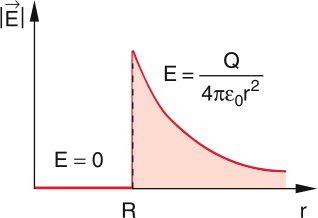
\includegraphics[width=5cm]{image/1/6.1}
    \end{minipage}
    \hspace{2cm}
    \begin{minipage}[b]{0.3\textwidth}
        \centering
        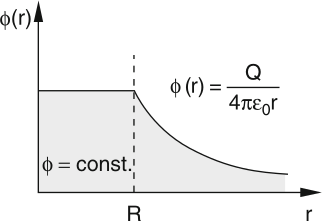
\includegraphics[width=5cm]{image/1/6.2}
    \end{minipage}
\end{figure}

\paragraph{Leiten Sie mit Hilfe des Gauß‘schen Gesetzes einen Ausdruck für das elektrische Feld und
das elektrostatische Potenziale eines homogen geladenen Kugelvolumens her. Erstellen Sie
ein Diagramm der beiden Größen als Funktion des Zentrumsabstandes.} ~

\begin{equation}
    \oint_{A} \bold{E} d\bold{A}
    = \frac{Q}{\epsilon_0}
    \implies
    \bold{E(r)} =
    \begin{cases}
        \frac{Q r}{4 \pi \epsilon_0 R^3} \bold{\hat{r}} ~für~ r<R \\
        \frac{Q}{4 \pi \epsilon_0 r^2} \bold{\hat{r}} ~für~ r>R
    \end{cases}
\end{equation}
\begin{equation}
    \phi(\bold{r})
    = \int_{\bold{r}}^\infty \bold{E} d\bold{s}
    = \begin{cases}
        \frac{Q}{4 \pi \epsilon_0 R} \left( \frac{3}{2} - \frac{r^2}{2 R^2} \right) ~für~ r<R \\
        \frac{Q}{4 \pi \epsilon_0 r} ~für~ r>R
    \end{cases}
\end{equation}

\begin{figure}[H]
    \centering
    \begin{minipage}[b]{0.3\textwidth}
        \centering
        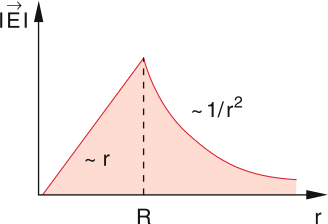
\includegraphics[width=5cm]{image/1/7.1}
    \end{minipage}
    \hspace{2cm}
    \begin{minipage}[b]{0.3\textwidth}
        \centering
        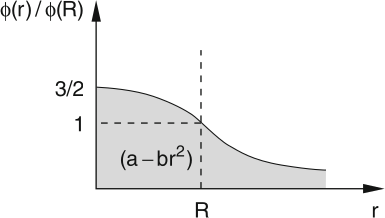
\includegraphics[width=5cm]{image/1/7.2}
    \end{minipage}
\end{figure}

\paragraph{Leiten Sie mit Hilfe des Gauß‘schen Gesetzes einen Ausdruck für das elektrische Feld und
das elektrostatische Potenziale einer homogen geladenen, sehr langen Zylinderfläche her.
Erstellen Sie ein Diagramm der beiden Größen als Funktion des Zentrumsabstandes.} ~

\begin{equation}
    \oint_{A} \bold{E} d\bold{A}
    = \frac{Q}{\epsilon_0}
    = \frac{\lambda l}{\epsilon_0}
    = E(r) \cdot 2 \pi r l
    \implies
    E(r) =
    \begin{cases}
        0 ~für~ r<R \\
        \frac{\lambda}{2 \pi \epsilon_0 r} ~für~ r>R
    \end{cases}
\end{equation}
\begin{equation}
    \phi(r)
    = \int_{r}^R E ds
    = \begin{cases}
        0 ~für~ r<R \\
        \frac{\lambda}{2 \pi \epsilon_0} \cdot ln \left( \frac{R}{r} \right) ~für~ r>R
    \end{cases}
\end{equation}

Als Potentialreferenz wird hierbei $R$ anstatt $\infty$ verwendet.

\begin{figure}[H]
    \centering
    \begin{minipage}[b]{0.3\textwidth}
        \centering
        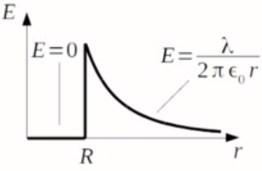
\includegraphics[height=3cm]{image/1/8.1}
    \end{minipage}
    \hspace{2cm}
    \begin{minipage}[b]{0.3\textwidth}
        \centering
        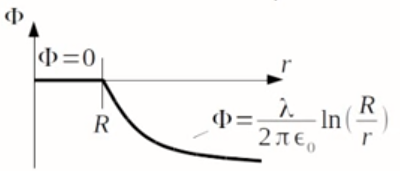
\includegraphics[height=3cm]{image/1/8.2}
    \end{minipage}
\end{figure}

\paragraph{Leiten Sie mit Hilfe des Gauß‘schen Gesetzes einen Ausdruck für das elektrische Feld und
das elektrostatische Potenziale eines homogen geladenen, sehr langen Zylindervolumnes
her. Erstellen Sie ein Diagramm der beiden Größen als Funktion des Zentrumsabstandes.} ~

\begin{equation}
    \oint_{A} \bold{E} d\bold{A}
    = \frac{Q}{\epsilon_0}
    = \frac{\lambda l}{\epsilon_0}
    = E(r) \cdot 2 \pi r l
    \implies
    E(r) =
    \begin{cases}
        \frac{\lambda r}{2 \pi \epsilon_0 R^2} ~für~ r<R \\
        \frac{\lambda}{2 \pi \epsilon_0 r} ~für~ r>R
    \end{cases}
\end{equation}
\begin{equation}
    \phi(r)
    = \int_{r}^R E ds
    = \begin{cases}
        \frac{\lambda}{4 \pi \epsilon_0} \cdot (1 - \frac{r^2}{R^2}) ~für~ r<R \\
        \frac{\lambda}{2 \pi \epsilon_0} \cdot ln \left( \frac{R}{r} \right) ~für~ r>R
    \end{cases}
\end{equation}

Als Potentialreferenz wird hierbei $R$ anstatt $\infty$ verwendet.

\begin{figure}[H]
    \centering
    \begin{minipage}[b]{0.3\textwidth}
        \centering
        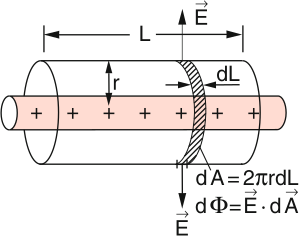
\includegraphics[width=5cm]{image/1/9.1}
    \end{minipage}
    \hspace{2cm}
    \begin{minipage}[b]{0.3\textwidth}
        \centering
        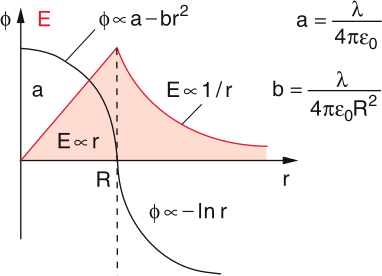
\includegraphics[width=5cm]{image/1/9.2}
    \end{minipage}
\end{figure}

\paragraph{Leiten Sie mit Hilfe des Gauß‘schen Gesetzes einen Ausdruck für das elektrische Feld und
das elektrostatische Potenzial einer homogen geladenen, unendlich großen, ebenen Fläche
her. Erstellen Sie ein Diagramm der beiden Größen als Funktion des Abstandes von der
Fläche.} ~

\begin{equation}
    \phi = 2 A E = \frac{Q}{\epsilon_0} = \frac{\sigma A}{\epsilon_0}
    \implies
    E = sgn(z) \cdot \frac{\sigma}{2 \epsilon_0}
\end{equation}
\begin{equation}
    \phi = \int_{z}^0 E ds = - E \cdot z = - \frac{\sigma}{2 \epsilon_0} \cdot |z|
\end{equation}

Als Potentialreferenz wird hierbei $0$ anstatt $\infty$ verwendet.

\begin{figure}[H]
    \centering
    \begin{minipage}[b]{0.3\textwidth}
        \centering
        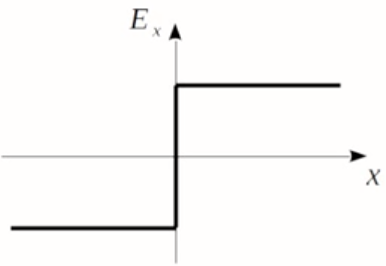
\includegraphics[width=5cm]{image/1/10.1}
    \end{minipage}
    \hspace{2cm}
    \begin{minipage}[b]{0.3\textwidth}
        \centering
        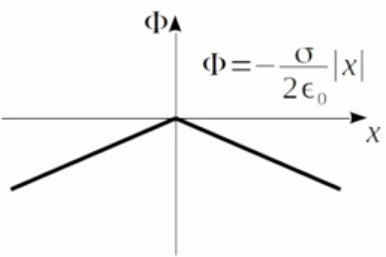
\includegraphics[width=5cm]{image/1/10.2}
    \end{minipage}
\end{figure}

\paragraph{Berechnen Sie das elektrische Feld einer Anordnung aus zwei sehr großen, parallelen,
homogen geladenen ebenen Flächen mit unterschiedlicher Flächenladungsdichte und
endlichem Abstand.} ~

\begin{equation}
    \text{eine Platte:} ~~~
    \phi = \frac{Q}{\epsilon_0} = \frac{\sigma A}{\epsilon_0} = \oint_A EdA = 2 E A
    \implies
    E = \frac{\sigma}{2 \epsilon_0}
\end{equation}
\begin{equation}
    \text{zwei Platten:} ~~~
    E_{ges}
    = E_1 + E_2
    = \frac{\sigma_1}{2 \epsilon_0} + \frac{\sigma_2}{2 \epsilon_0}
    = \frac{\sigma_1 + \sigma_2}{2 \epsilon_0}
\end{equation}

\paragraph{Berechnen Sie das elektrische Feld einer Anordnung aus zwei homogen geladenen
Kugelflächen mit unterschiedlicher Gesamtladung. Der Abstand der Kugelmittelpunkte ist
größer als die Summe der Kugelradien.} ~

\begin{equation}
    E(r)
    = E_1(r) + E_2(r)
    = \frac{Q_1}{4 \pi \epsilon_0 r^2} + \frac{Q_2}{4 \pi \epsilon_0 (d -r )^2}
\end{equation}

Dieser Zusammenhang gilt nur für $R_1 < r < d-R_2$.

\paragraph{Berechnen Sie die Kraft, das Drehmoment und die potenzielle Energie eines Dipols im
homogenen elektrischen Feld.} ~

\begin{equation}
    \bold{F} = \bold{F_1} + \bold{F_2} = Q\bold{E} - Q\bold{E} = 0
\end{equation}
\begin{equation}
    \bold{M}
    = Q (\bold{r_1} \times \bold{E}) - Q (\bold{r_2} \times \bold{E})
    = Q \bold{d} \times \bold{E}
    = \bold{p} \times \bold{E}
\end{equation}
\begin{equation}
    W_{pot} = Q (\phi_1 - \phi_2) = - \bold{p} \cdot \bold{E}
\end{equation}

\begin{figure}[H]
    \centering
    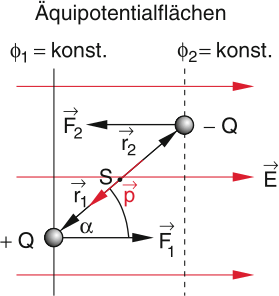
\includegraphics[width=5cm]{image/1/13}
\end{figure}

\paragraph{Berechnen Sie die Kraft auf einen Dipol in einem inhomogenen elektrischen Feld. Schreiben
Sie eine Näherung für diese Kraft für den Grenzfall eines sehr kleinen Dipols an.} ~

\begin{equation}
    \bold{F} = \bold{F_+} + \bold{F_-} = q [ \bold{E} (\bold{r_-} + \bold{d}) - \bold{E(r_-)}]
\end{equation}
\begin{equation}
    \bold{F} \approx Q \bold{d} \frac{d\bold{E(r)}}{d\bold{r}} = \bold{p} \nabla \bold{E(r)}
\end{equation}

\begin{figure}[H]
    \centering
    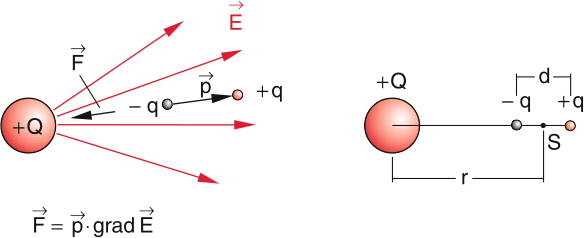
\includegraphics[width=8cm]{image/1/14}
\end{figure}

\newpage

\section{Materie im elektrischen Feld}

\paragraph{Was ist ein elektrischer Leiter und was passiert wenn ein elektrischer Leiter in ein
statisches elektrisches Feld gebracht wird. Wie nennt man den Effekt und welche Bedingungen muss das
elektrische Feld und -Potenzial an der Leiteroberfläche und innerhalb des Leiters erfüllen?} ~

Ein elektrischer Leiter ist ein Medium, welches eine hohe Dichte frei beweglicher Ladungsträger und
daher eine gute elektrische Leitfähigkeit sowie einen möglichst geringen elektrischen Widerstand
besitzt. Er ist dadurch zum Transport geladener Teilchen geeignet, welchen man auch als elektrischen
Strom bezeichnet.

Es kommt zu einer Ladungsverschiebung aufgrund des E-Feldes, wodurch sich ein Gegenfeld aufbaut und
das äußere Feld kompensiert. Das Innere des Leiters wird dadurch feldfrei, man spricht von Influenz.
Die beweglichen Ladungsträger befinden sich an der Leiteroberfläche und bilden somit eine
Äquipotentialfläche, auf welche die Feldlinien senkrecht stehen. Das Potential im Inneren des
Leiters ist konstant.

\paragraph{Was ist ein Kondensator? Warum kann man eindeutig eine elektrische Spannung zwischen zwei
entgegengesetzt geladenen Metallkörpern angeben? Wie ist die elektrische Kapazität definiert und
wovon hängt deren Größe ab?} ~

Ein Kondensator ist ein elektrisches Bauelement mit der Fähigkeit, elektrische Ladung und die damit
zusammenhängende Energie in einem elektrischen Feld zu speichern.

Da das elektrische Feld im Raum zwischen den Leiterflächen proportional zur Ladung $Q$ und die
Spannung $U$ wegen $U = \int \bold{E} d\bold{s}$ proportional zu $Q$ ist gilt die Beziehung
\begin{equation}
    C = \frac{Q}{U} \text{ ,}
\end{equation}
wobei die in Farad angegebene Proportionalitätskonstante $C$ die Kapazität des Kondensators ist.
Diese ist sowohl von der Geometrie als auch vom verwendeten Dielektrikum zwischen den Leitern
abhängig.

\paragraph{Ein Plattenkondensator mit der Kapazität $C$ und Plattenabstand $d_C$ ist auf die Spannung
$U$ geladen und von der Spannungsquelle getrennt. Nun wird eine isolierte Metallplatte (Dicke
$d_M<d_C$) parallel zu den Kondensatorplatten zwischen diese eingeschoben. Beschreiben Sie was
passiert. Berechnen Sie die elektrische Feldstärken vor- und nach Einschieben der Platte. Zeichnen
Sie ein Diagramm der elektrischen Feldstärke und des elektrischen Potenzials zwischen den
Kondensatorplatten vor und nach Einschieben der Metallplatte.} ~

Aufgrund der Influenz erfolgt eine Ladungsverschiebung in der Platte, auf dessen Oberfläche sich nun
die Ladungsträger sammeln und ein Gegenfeld bewirken, welches das Innere der Platte feldfrei macht.
Dadurch sinkt auch die Spannung, da effektiv weniger Plattenabstand vorhanden ist - die Kapazität
$C$ des Kondensators steigt.

\begin{equation}
    \text{vorher:} ~~~
    E_V = \frac{Q}{A \cdot \epsilon_0} = \frac{U}{d_C}
\end{equation}
\begin{equation}
    \text{nachher:} ~~~
    E_V = \frac{U}{d_C - d_M} ~~~
    E_M = 0
\end{equation}

\begin{figure}[H]
    \centering
    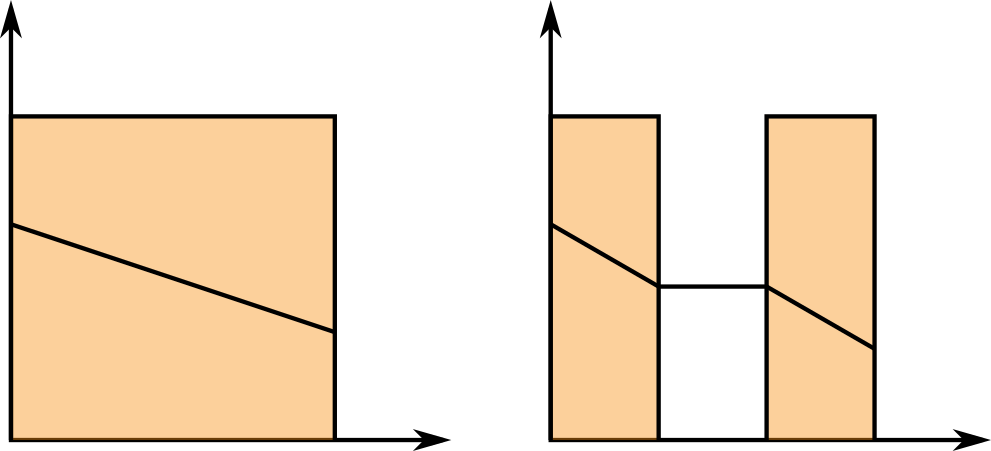
\includegraphics[width=5cm]{image/2/3}
\end{figure}

\paragraph{Ein Plattenkondensator mit der Kapazität $C$ und Plattenabstand $d_C$ ist an eine
Spannungsquelle mit der Spannung $U$ angeschlossen. Nun wird eine dielektrische Platte (Dicke $d_D$,
Permitivität $\epsilon_D$) parallel zu den Kondensatorplatten zwischen diese eingeschoben.
Beschreiben Sie was passiert. Berechnen Sie die elektrische Feldstärken und die elktrischen
Verschiebungsdichten vor- und nach einschieben der Platte. Zeichnen Sie ein Diagramm der
elektrischen Feldstärke, der dielektrischen Verschiebungsdichte und des elektrischen Potenzials
zwischen den Kondensatorplatten vor und nach Einschieben der dielektrischen Platte.} ~

Durch das Feld des Kondensators werden die festen Moleküle im Dielektrikum polarisiert - es bildet
sich ein Gegenfeld, welches das äußere jedoch nicht vollständig kompensiert. Die Feldstärke und die
Spannung sinken um den Faktor $\epsilon_D$, die Kapazität steigt entsprechend um den Faktor
$\epsilon_D$.

\begin{equation}
    \text{vorher:} ~~~
    E_V = \frac{Q}{A \cdot \epsilon_0} = \frac{U}{d_C} ~~~
    D_V = E_V \cdot \epsilon_0
\end{equation}
\begin{equation}
    \text{nachher:} ~~~
    E_V = \frac{U}{d_C - d_D + \frac{d_D}{\epsilon_D}} ~~~
    E_D = \frac{E_V}{\epsilon_D} ~~~
    D_V = D_D
\end{equation}

\begin{figure}[H]
    \centering
    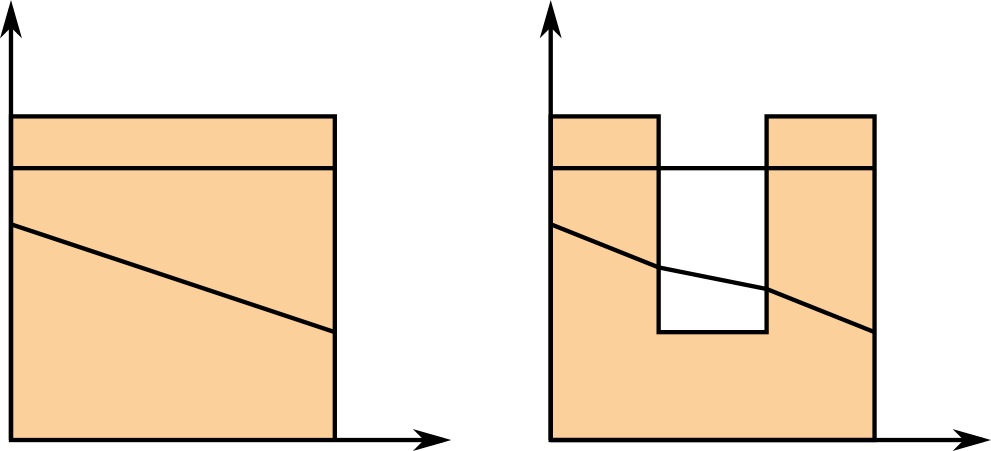
\includegraphics[width=5cm]{image/2/4}
\end{figure}

\paragraph{Ein Plattenkondensator mit Fläche $A$, Plattenabstand $d$, gefüllt mit einem Dielektrikum
mit der relativen Permittivität $\epsilon$ ist mit der Ladung $Q$ geladen. Wie groß ist die in ihm
gespeicherte Energie?}

\begin{equation}
    E_{el} = \frac{Q^2}{2 \cdot C} = \frac{Q^2}{2 \cdot \epsilon \epsilon_0 \frac{A}{d}}
\end{equation}

\paragraph{Was ist der Unterschied zwischen Polarisation und Influenz? Welche Arten von Polarisation
können bei einem Dielektrikum auftreten? Was für Voraussetzungen müssen die Moleküle des
Dielektrikums dafür erfüllen?} ~

Unter Influenz versteht man die räumliche Verschiebung frei beweglicher Ladungsträger im Leiter
durch ein äußeres Feld, wodurch sich ein (meist das äußere Feld kompensierendes) Gegenfeld bildet.
Die Polarisation ist ein vergleichbarer Effekt im Dielektrikum, allerdings können hier die Ladungen
nur innerhalb der Atome oder Moleküle verschoben werden. Es entsteht ein schwächeres Gegenfeld als
im Leiter, das äußere Feld kann nicht kompensiert werden.

\begin{itemize}
    \item Induzierte Polarisation: Die Polarisierbarkeit (Verschiebbarkeit der negativen und
    positiven Ladungsträger im Atom oder Molekül relativ zueinander) muss ausreichend groß sein.
    
    \item Orientierungspolarisation: Die Schwerpunkte der positiven und negativen Ladungen müssen
    deutlich voneinander getrennt sein, man spricht von Dipolmolekülen oder permanenten Molekülen.
    Ein Beispiel hierfür sind Wassermoleküle.
\end{itemize}

\paragraph{Beschreiben Sie die Größen elektrische Polarisation, Suzeptibilität,
Dielektrizitätskonstante, dielektrische Verschiebungsdichte und elektrische Feldstärke. Wie hängen
sie zusammen und welche Einheiten haben sie?}

\begin{itemize}
    \item Polarisation $\bold{P}$: Beschreibt, wie stark ein Dielektrikum polarisiert ist
    beziehungsweise kennzeichnet die Stärke des Dipolmoments in dielektrischen Material.
    $[P] = \si{\A\s\per\m^2}$
    
    \item Suszeptibilität (Reizbarkeit) $\chi$: Materialeigenschaft, welche die Fähigkeit zur
    elektrischen Polarisierung in einem eingeprägten elektrischen Feld angibt. $[\chi] = 1$
    
    \begin{equation}
        \chi = \frac{P}{E \cdot \epsilon_0}
    \end{equation}
    
    \item Dielektrizitätskonstante $\epsilon$: Gibt die Polarisationsfähigkeit eines Materials
    durch elektrische Felder an. $[\epsilon] = \si{\A\s\per\V\per\m}$
    
    \item Dielektrische Verschiebungsdichte $\bold{D}$: Ist ein Maß für die auf einer Fläche im
    elektrischen Feld durch Influenz hervorgerufenen Ladung. $[D] = \si{\coulomb\per\m^2}$
    
    \begin{equation}
        \bold{D} = \epsilon \epsilon_0 \bold{E} = \epsilon_0 \bold{E} + \bold{P}
    \end{equation}
    
    \item Elektrische Feldstärke $\bold{E}$: Beschreibt die Stärke und Richtung eines elektrischen
    Feldes, also die Fähigkeit des Feldes, Kraft auf Ladungen auszuüben. $[E] = \si{\V\per\m}$
\end{itemize}

\paragraph{Schreiben Sie die Feldgleichungen der Elektrostatik in Materie an (Integralform) und
benennen Sie alle vorkommenden Größen inklusive Einheiten.}

\begin{equation}
    \oint_A \bold{E} d\bold{A} = \frac{Q}{\epsilon_0} ~~~ \oint \bold{E} d\bold{s} = 0
\end{equation}

\begin{itemize}
    \item $A$: Oberfläche des Volumens $[A] = \si{\m^2}$
    \item $\bold{E}$: Elektrische Feldstärke $[E] = \si{\V\per\m}$
    \item $Q$: Eingeschlossene Ladung $[Q] = \si{\coulomb}$
    \item $\epsilon_0$: Elektrische Feldkonstante $[\epsilon_0] = \si{\A\s\per\V\per\m}$
\end{itemize}

\paragraph{Ein Elektron bewegt sich zum Zeitpunkt $t_0$ mit der Geschwindigkeit $v_0$ senkrecht zu
den elektrischen Feldlinien in einem elektrischen Feld. Stellen Sie die Bewegungsgleichung auf und
beschreiben Sie die weitere Bahn des Elektrons.}

\begin{equation}
    F = q \cdot E = m \cdot a_y
    \implies
    a_y = \frac{E \cdot e}{m}
\end{equation}
\begin{equation}
    s_x(t) = v_0 \cdot t
\end{equation}
\begin{equation}
    s_y(t) = \frac{1}{2} \cdot a_y \cdot t^2
\end{equation}

Außerhalb des Feldes gilt für die Beschleunigung $a_y = 0$, die weitere Kurve entspricht einer
Geraden.

\paragraph{Beschreiben Sie Zweck und Funktionsprinzip des Millikan Versuches. Wie kann die Masse und
die elektrostatische Kraft auf die Öltröpfchen bestimmt werden und wie bestimmt man deren Ladung?} ~

Der Millikan-Versuch dient der experimentellen Ermittlung der Elementarladung $e$. Durch Zerstäuben
von Öl werden kleine Öltröpfchen erzeugt, welche aufgrund der Reibung beim Zerstäubungsvorgang die
Ladung $n \cdot e$ besitzen und zwischen die horizontalen Platten eines Kondensators diffundieren.

Im feldfreien Kondensator wird die Schwerkraft $m \cdot g$ durch die Summe der Auftriebskraft
$F_A = \rho_{Luft} \cdot \frac{4}{3} \pi R^3 \cdot g$ und der Reibungskraft
$F_R = 6 \pi \eta R \cdot v$ kompensiert. Die sich einstellende konstante Sinkgeschwindigkeit kann
gemessen werden, wodurch sich der Radius und in weiterer Folge die Masse des Tröpfchens ergeben.

Durch Anlegen einer geeigneten Spannung am Kondensator kann nun das Tröpfchen im E-Feld in Schwebe
gehalten werden. Eine Ladungsänderung des Tröpfchens durch beispielsweise Röntgenstrahlung erfordert
eine Spannungsänderung, um den Schwebezustand aufrecht zu erhalten. Mithilfe der bekannten
Spannungswerte kann nun $n$ und in weiterer Folge $e$ bestimmt werden.

\begin{figure}[H]
    \centering
    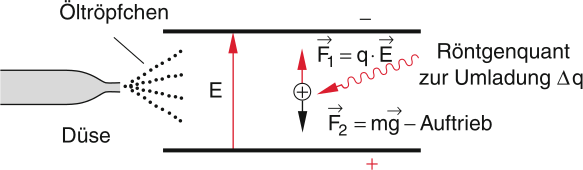
\includegraphics[width=10cm]{image/2/10}
\end{figure}

\newpage

\section{Elektrischer Strom I}

\paragraph{Was bedeuten die Begriffe elektrischer Strom, Stromdichte und Driftgeschwindigkeit und
wie sind sie miteinander verknüpft? Welche Einheiten habe diese Größen? Sind es skalare oder
vektorielle Grössen?} ~

\begin{itemize}
    \item Elektrischer Strom $I$: Transport von elektrischen Ladungsträgern $[I] = \si{\A}$
        \begin{equation}
            I = \int_A \bold{j} d\bold{A}
        \end{equation}
    
    \item Stromdichte $\bold{j}$: Verhältnis der Stromstärke $I$ zur Verfügung stehenden
        Querschnittsfläche $A$ $[j] = \si{\A\per\m^2}$
        \begin{equation}
            \bold{j} = n \cdot q \cdot \bold{v_D} 
        \end{equation}
    
    \item Driftgeschwindigkeit $\bold{v_D}$: Die mittlere Geschwindigkeit der Ladungsträger aufgrund
        eines äußeren Feldes $[v] = \si{\m\per\s}$
\end{itemize}

\paragraph{Was bedeuten die Begriffe Beweglichkeit und elektrische Leitfähigkeit und spezifischer
Widerstand? Welche Einheit haben sie und in welcher Beziehung stehen sie zur Stromdichte?} ~

\begin{itemize}
    \item Beweglichkeit $\mu$: Gibt die Driftgeschwindigkeit der Ladungsträger bei einer
        elektrischen Feldstärke von \SI{1}{\V\per\m} an $[\mu] = \si{\m\squared\per\V\per\s}$
        \begin{equation}
            \bold{j} = \sigma \cdot \frac{\bold{v_D}}{\mu}
        \end{equation}
    
    \item Elektrische Leitfähigkeit $\sigma$: Fähigkeit eines Stoffes, den elektrischen Strom zu
        leiten $[\sigma] = \si{\A\per\V\per\m}$
        \begin{equation}
            \bold{j} = \sigma \cdot \bold{E}
        \end{equation}
    
    \item Spezifischer Widerstand $\rho_s$: Kehrwert der elektrischen Leitfähigkeit
        $[\rho_s] = \si{\ohm\m}$
        \begin{equation}
            \bold{E} = \rho_s \cdot \bold{j}
        \end{equation}
\end{itemize}

\paragraph{Was besagt das Ohm‘sche Gesetz? Schreiben Sie das Ohm‘sche Gesetz in seiner lokalen und
integralen Form an. Was ist ein Ohm‘scher Leiter?} ~

Die Stärke des durch ein Objekt fließenden elektrischen Stroms ist proportional der elektrischen
Spannung.
\begin{equation}
    \bold{j} = \sigma \cdot \bold{E} ~~~ I = \frac{\sigma_{el} \cdot A}{L} \cdot U = \frac{U}{R}
\end{equation}
Einen Leiter, für welchen $\rho_s$ unabhängig von Strom $I$ und Spannung $U$ sind, nennt man
ohm'schen Leiter. Die Spannung $U$ und der Strom $I$ sind also über $R$ proportional zueinander.

\paragraph{Eine ideale Spannungsquelle liefert eine Klemmspannung von \SI{10}{\V}. Entwerfen und
dimensionieren Sie eine einfache Schaltung aus Widerständen, die es ihnen erlaubt eine Spannung von
\SI{4}{\V} abzugreifen. Der gesamtwiderstand der Schaltung sollte \SI{10}{\kilo\ohm} sein.}

\begin{equation}
    I = \frac{U_0}{R_{ges}} = \frac{U_1}{R_1} = \frac{U_2}{R_2}
\end{equation}
\begin{equation}
    \begin{rcases}
        R_1 = R_{ges} \cdot \frac{U_1}{U_0} \\
        R_2 = R_1 \cdot \frac{U_2}{U_1}
    \end{rcases}
    \implies
    R_2 = R_{ges} \cdot \frac{U_2}{U_0} = \SI{4}{\kilo\ohm}
\end{equation}
\begin{equation}
    R_1 = R_{ges} - R_1 = \SI{6}{\kilo\ohm}
\end{equation}

\begin{figure}[H]
    \centering
    \includegraphics[width=5cm]{image/3/4}
\end{figure}

\paragraph{Das Material eines metallischen Leiters (Draht) mit konstanter Querschnittsfläche $F$ und
einer Länge $L$, habe den spezifischen Widerstand $\rho$. Berechnen Sie den Ohm‘schen Widerstand des
Drahtes.} ~
\begin{equation}
    R = \rho \cdot \frac{L}{F}
\end{equation}

\paragraph{Beschreiben Sie den Ladungsvorgang eines Kondensators, der über einen Widerstand
plötzlich mit einer idealen Spannungsquelle verbunden wird (Strom und Spannungen als Funktion der
Zeit).} ~

\begin{equation}
    U(t) = U_0 \cdot \left( 1 - e^{-t /(R C)} \right)
\end{equation}
\begin{equation}
    I(t) = I_0 \cdot e^{-t /(R C)}
\end{equation}

\begin{figure}[H]
    \centering
    \begin{minipage}[b]{0.3\textwidth}
        \centering
        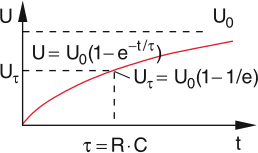
\includegraphics[width=5cm]{image/3/6.1}
    \end{minipage}
    \hspace{2cm}
    \begin{minipage}[b]{0.3\textwidth}
        \centering
        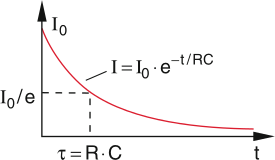
\includegraphics[width=5cm]{image/3/6.2}
    \end{minipage}
\end{figure}

\paragraph{Beschreiben Sie den Entladungsvorgang eines geladenen Kondensators, dessen Kontakte über
einen Widerstand plötzlich verbunden werden (Strom und Spannungen als Funktion der Zeit).} ~

\begin{equation}
    U(t) = U_0 \cdot e^{-t /(R C)}
\end{equation}
\begin{equation}
    I(t) = I_0 \cdot e^{-t /(R C)}
\end{equation}

\begin{figure}[H]
    \centering
    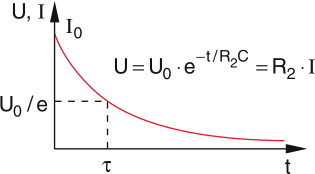
\includegraphics[width=5cm]{image/3/7}
\end{figure}

\paragraph{Beschreiben Sie die elektrische Leitung in Metallen. Wie ändert sich der spezifische
Widerstand mit der Temperatur? Begründen Sie.} ~

Das Anlegen einer Spannung bewirkt ein elektrisches Feld im Metall, welches die Elektronen zum
positiven Pol der Spannungsquelle hin beschleunigt. Duch die Kollision der Elektronen mit den Ionen
im Kristallgitter verlieren erstere kinetische Energie, welche in Wärmeenergie umgewandelt wird.

Bei höheren Temperaturen kommt es zu stärkeren Schwingungen der Metallionen, wodurch die Bewegung
der Elektronen noch stärker beschränkt wird. Der spezifische Widerstand steigt also mit der
Temperatur.

Bei sehr tiefen Temperaturen können viele Metalle ihren Widerstand völlig verlieren, man spricht
dann von Supraleitung.

\paragraph{Beschreiben Sie die elektrische Leitung in Halbleitern. Wie ändert sich der spezifische
Widerstand mit der Temperatur? Begründen Sie.} ~

Die Atome im Halbleiter bilden stabile Elektronenpaarbindungen, bei tiefen Temperaturen sind also
keine freien Elektronen verfügbar. Mit steigender Temperatur können aufgrund ihres höheren
Energie-Niveaus jedoch Elektronen frei werden, die Leitfähigkeit steigt also während der elektrische
Widerstand mit steigender Temperatur sinkt.

Durch das Fehlen von Elektronen im Gitter entstehen Löcher, welche als positive Ladungsträger
betrachtet werden können. Diese Löcher werden durch von Loch zu Loch springende Elektronen gefüllt,
wodurch sie scheinbar in entgegengesetzter Richtung der Elektronen wandern und damit ebenso dem
Ladungstransport dienen.

\paragraph{Beschreiben Sie die elektrische Leitung in Gasen.} ~

Der Ladungstransport in ionisierten Gasen, die auch als Plasma bezeichnet werden, erfolgt sowohl
durch Elektronen als auch durch Ionen. Neben der Existenz dieser frei beweglichen Ladungsträger ist
ein elektrisches Feld Voraussetzung für die Leitung in Gasen.

Die Erzeugung von Ladungsträgern im Gas kann über verschiedene Methoden erfolgen:

\begin{itemize}
    \item Thermische Ionisation: Durch eine Kombination der thermischen Anregung und der damit
        initiierten chemischen Prozesse entstehen Ladungsträger. Die erforderliche, sehr hohe
        Temperatur kann durch Verwendung eines Katalysators verringert werden.
    
    \item Elektronenstoßionisation: Elektronen mit ausreichend hoher Energie können beim Stoß mit
        Atomen oder Molekülen Elektronen aus der Elektronenhülle herausschlagen und damit ein
        Elektron-Ion-Paar bilden.
    
    \item Photoionisation: Durch kurzwellige Strahlung wie etwa UV- oder Röntgenstrahlung können
        Atome oder Moleküle aufgrund der hochenergetischen Photonen ihrer Elektronen beraubt werden.
        Dies führt ebenfalls zur Entstehung von Elektron-Ion-Paaren.
\end{itemize}

\paragraph{Beschreiben Sie die Ionenleitung in Flüssigkeiten.} ~

Flüssigkeiten, in denen Säuren, Laugen oder Salze gelöst sind, nennt man Elektrolyte. Im Gegensatz
zu Metallen ist hier der Stromdurchgang mit einer chemischen Zersetzung des Elektrolyten verbunden.
Sowohl an der Anode als auch an der Kathode werden Stoffe in fester oder gasförmiger Form
abgeschieden.

Durch Dissoziation - also durch Aufspaltung von Molekülen in kleinere Bestandteile - entstehen
positiv und negativ geladene Ionen. Diese ermöglichen bei einer angelegten Spannung den
Ladungstransport mit der sogenannten Driftgeschwindigkeit. Während die positiven Ionen zur Kathode
wandern und dort Elektronen aufnehmen geben die negativen Ionen an der Anode ihre überschüssigen
Elektronen ab. Dabei scheiden sie als neutrale Atome an der jeweiligen Elektrode ab.

\begin{figure}[H]
    \centering
    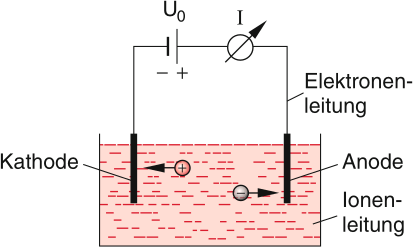
\includegraphics[width=7cm]{image/3/11}
\end{figure}

\newpage

\section{Elektrischer Strom II}

\paragraph{Beschreiben Sie die Funktionsweise eines galvanischen Elementes. Wodurch ist die
erzielbare Spannung bestimmt?} ~

Das Prinzip einer galvanischen Zelle beruht darauf, dass unterschiedliche Metalle eine
unterschiedliche Tendenz aufweisen, Elektronen abzugeben. Die Potentialdifferenz und damit auch die
abgreifbare Spannung sind umso größer, je unterschiedlicher die einzelnen Elementein dieser Hinsicht
sind.

Werden zwei Metallelektroden in eine gemeinsame Elektrolytlösung getaucht, so gibt eine der
Elektroden Metallionen an das Elektrolyt ab während die Elektronen auf der Elektrode zurückbleiben.
Von dem mit Ionen angereicherten Elektrolyt werden wiederum Metallionen auf die andere Elektrode
übertragen und dort entladen. Werden die Elektroden über einen elektrischen Leiter verbunden, so
können die Elektronen von einer Elektrode auf die andere übertragen werden. Die Reaktion läuft so
lange ab, bis sich die Elektrode aufgelöst hat.

Neben den verwendeten Metallen hängt die abgreifbare Spannung auch vom Elektrolyt ab.

\begin{figure}[H]
    \centering
    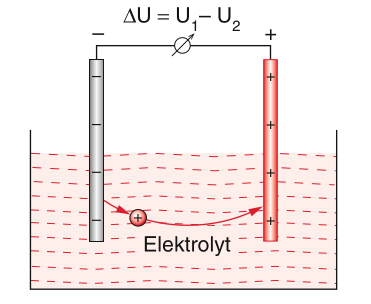
\includegraphics[width=4cm]{image/4/1}
\end{figure}

\paragraph{Beschreiben Sie die Funktionsweise einer Brennstoffzelle.} ~

Brennstoffzellen ermöglichen die direkte Umwandlung von chemischer in elektrische Energie ohne den
Umweg über Wärmeenergie.

Durch geschickte Konstruktion werden die Oxidations- sowie Reduktionsreaktion von Sauerstoff mit dem
verwendeten Brennstoff (wie etwa Wasserstoff) räumlich getrennt. Durch beispielsweise poröse, mit
Katalysatorstoffen versehene Elektroden im gemeinsamen Elektrolyt wird kontinuierlich Sauerstoff und
Wasserstoff zugeführt. Die beiden Reaktionen laufen dann getrennt an der jeweiligen Elektrode ab.

Der Wasserstoff an der Anode zerfüllt durch die katalytische Wirkung schon bei Raumtemperatur in
Protonen und Elektronen. Die Protonen gelangen durch das Elektrolyt auf die Kathodenseite. Die
Elektronen wandern durch den geschlossenen äußeren Stromkreis zur Kathode und verrichten auf diesem
Wege elektrische Arbeit. An der Kathode verbinden sich Protonen, Elektronen und Sauerstoff zu
Wasser.

\begin{figure}[H]
    \centering
    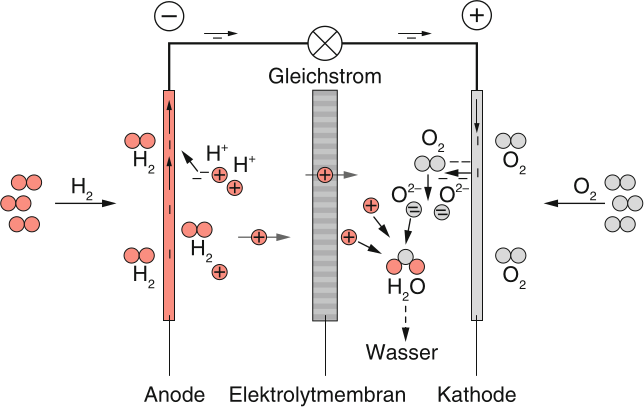
\includegraphics[width=7cm]{image/4/2}
\end{figure}

\paragraph{Beschreiben Sie den Seebeck-Effekt und die Ursache der Thermospannung.} ~

Werden zwei Leiter unterschiedlicher Stoffe zu einem geschlossenen Stromkreis verlötet, so misst man
bei unterschiedlichen Temperaturen der Lötstellen eine Spannung. Man spricht vom Seebeck-Effekt.

Am heißen Ende des Leiters gibt es mehr Elektronen mit hoher Energie und weniger Elektronen mit
geringer Energie. Durch Diffusion bewegen sich die energiereichen Elektronen zum kalten Ende und
Elektronen mit wenig Energie zum heißen Ende. Das entstehende Ungleichgewicht wird durch ein
elektrisches Feld ausgeglichen, die entstehende Spannung ist die Seebeck-Spannung.

\begin{figure}[H]
    \centering
    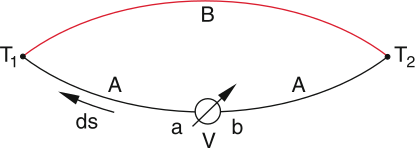
\includegraphics[width=6cm]{image/4/3}
\end{figure}

\paragraph{Was ist der Innenwiderstand einer Spannungsquelle? Wie groß ist der Innenwiderstand einer
idealen Spannungsquelle bzw. einer idealen Stromquelle?} ~

Der Innenwiderstand $R_i$ einer Spannungsquelle rührt daher, dass die Ladungsträger auf dem Weg vom
Ort ihrer Trennung bis zu den Ausgangsklemmen der Quelle Stöße mit Atomen oder Molekülen innerhalb
der Quelle erleiden.

Der Innenwiderstand einer idealen Spannungsquelle ist \SI{0}{\ohm}, der einer idealen Stromquelle
$\infty~\si{\ohm}$.

\begin{figure}[H]
    \centering
    \begin{minipage}[b]{0.3\textwidth}
        \centering
        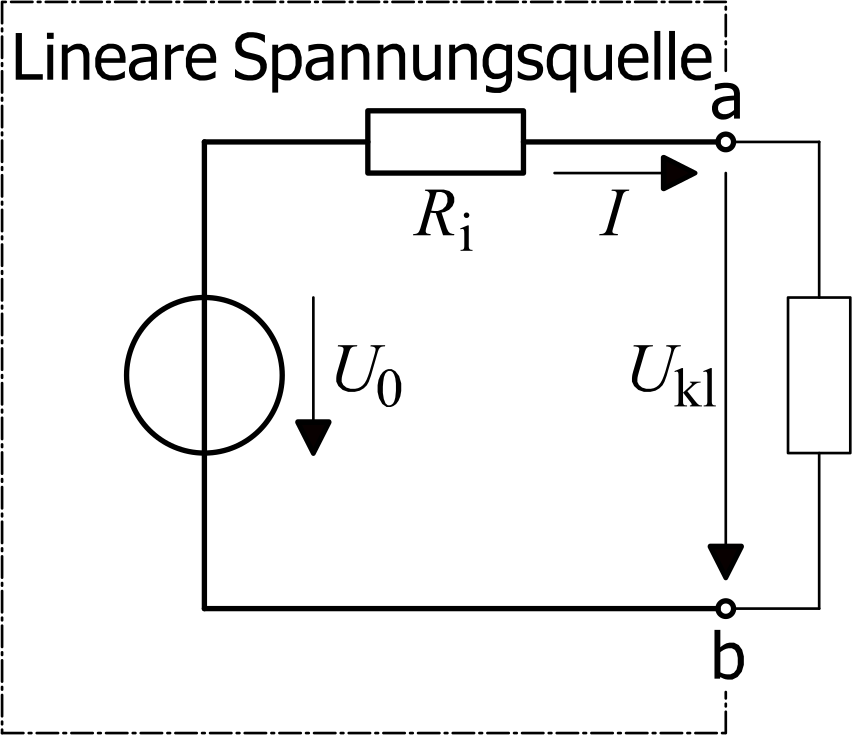
\includegraphics[width=4cm]{image/4/4.1}
    \end{minipage}
    \hspace{2cm}
    \begin{minipage}[b]{0.3\textwidth}
        \centering
        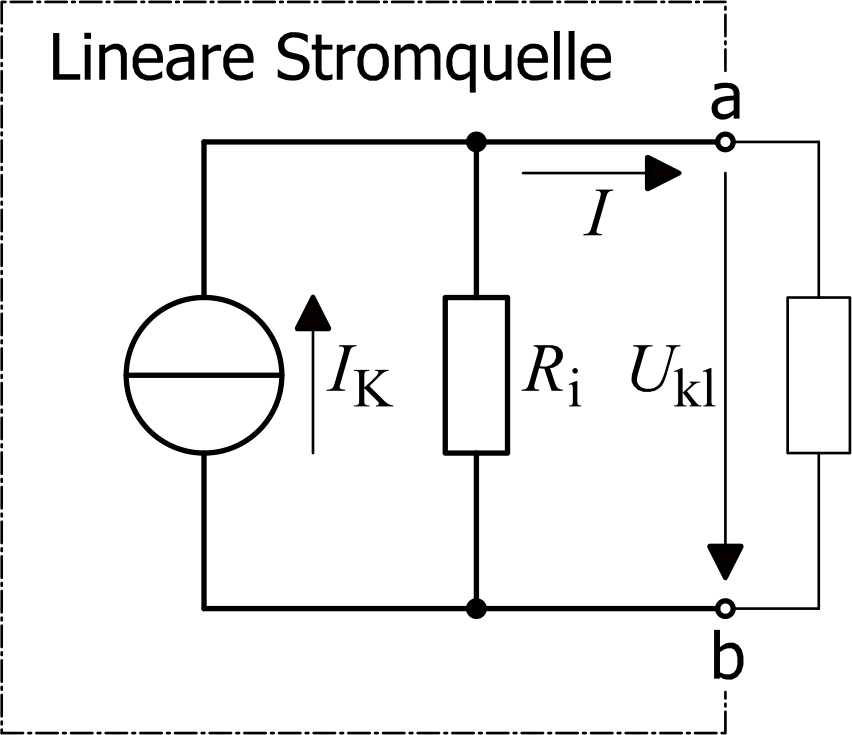
\includegraphics[width=4cm]{image/4/4.2}
    \end{minipage}
\end{figure}

\paragraph{Wie kann man den Kurzschlussstrom und den Innenwiderstand eines Akkumulators durch
Strom und Spannungsmessung ermitteln, ohne den Akku wirklich kurz zu schließen? Der Akkumulator sei
in guter Näherung eine lineare Spannungsquelle. Schaltungsskizze!} ~

\begin{enumerate}
    \item Leerlaufspannung $U_0$ direkt per Voltmeter messen
    
    \item Potentiometer als Lastwiderstand schalten und derart einstellen, dass genau die Hälfte
        der Leerlaufspannung am Potentiometer abfällt. Der nun am Potentiometer eingestellte Wert
        entspricht genau dem des Innenwiderstandes $R_i$.
    
    \item Der Kurzschlussstrom ergibt sich mit $I_K = \frac{U_0}{R_i}$
\end{enumerate}

\begin{figure}[H]
    \centering
    \begin{minipage}[b]{0.3\textwidth}
        \centering
        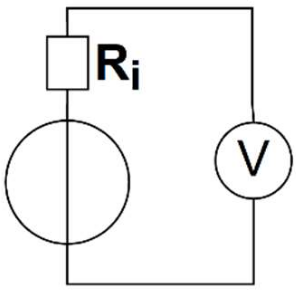
\includegraphics[height=3cm]{image/4/5.1}
    \end{minipage}
    \hspace{2cm}
    \begin{minipage}[b]{0.3\textwidth}
        \centering
        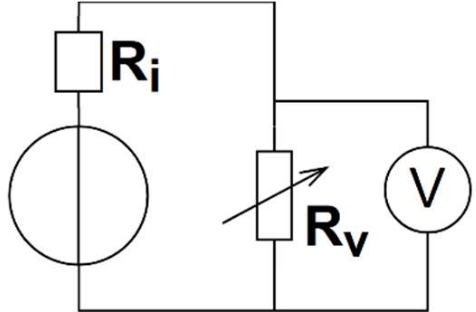
\includegraphics[height=3cm]{image/4/5.2}
    \end{minipage}
\end{figure}

\paragraph{Zeichnen Sie das Ersatzschaltbild einer mit einem Widerstand $R$ belasteten linearen
Spannungsquelle mit Innenwiderstand $R_i$ und elektromotorischer Kraft $U$. Berechnen Sie einen
Ausdruck für die Klemmspannnung.} ~

\begin{equation}
    U_K = U_0 - R_i \cdot I = U_0 - R_i \cdot \frac{U_0}{R_i + R}
\end{equation}

\begin{figure}[H]
    \centering
    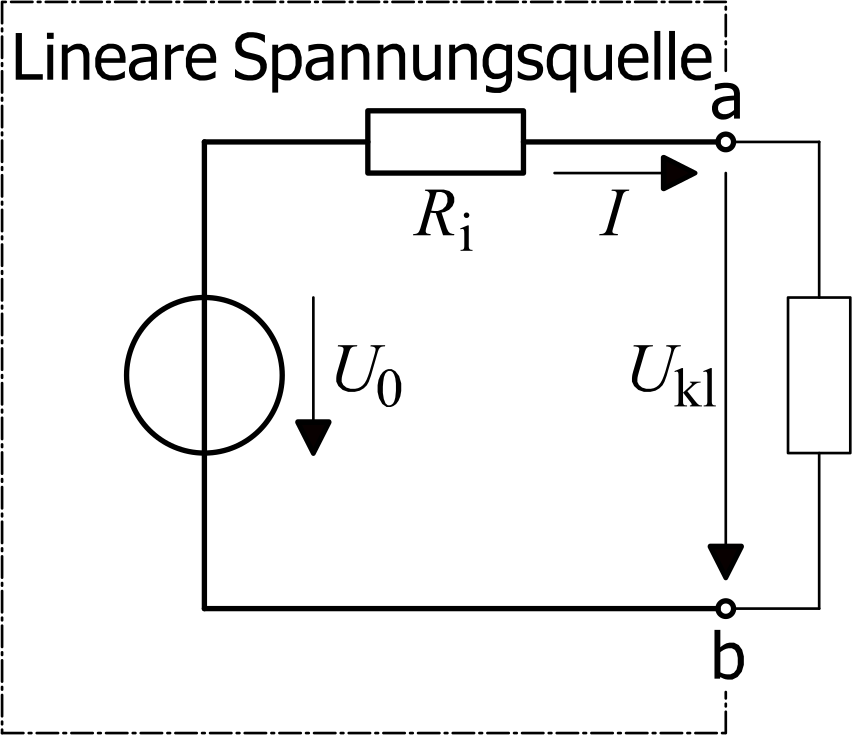
\includegraphics[width=5cm]{image/4/6}
\end{figure}

\paragraph{Was versteht man unter Leistungsanpassung bei einer Spannungsquelle? Bei welchem Last-
bzw. Innenwiderstand ist dies erfüllt?} ~

Unter Leistungsanpassung versteht man die Dimensionierung des Innen- und Lastwiderstandes, sodass
die im Verbraucher umgesetzte Leistung maximal wird. Dies ist der Fall, wenn $R_i = R_L$ gilt.

\begin{figure}[H]
    \centering
    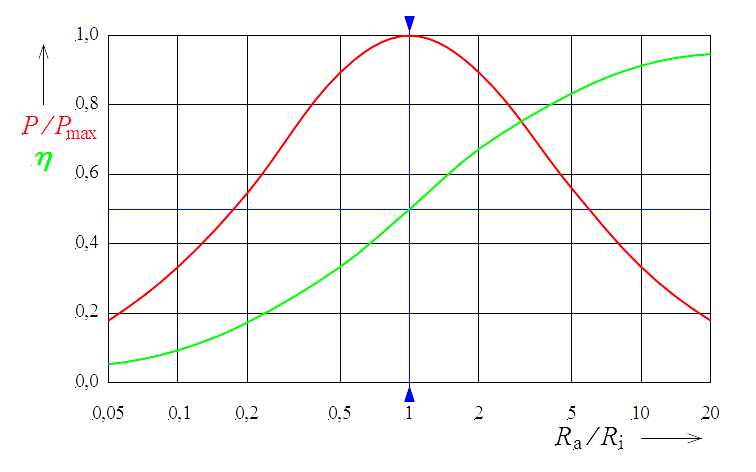
\includegraphics[width=8cm]{image/4/7}
\end{figure}

\paragraph{Beschreiben und erklären Sie die Funktionsweise eines Dual-Slope Analog-Digital
Umsetzers.} ~

Ein Analog-Digital-Umsetzer ist eine elektronisches Gerät zur Umsetzung analoger Eingangssignale in
einen digitalen Datenstrom. Die Eingangsgröße ist dabei immer eine elektrische Spannung.

Beim Dual-Slope-Verfahren wird ein Kondensator während einer Integrationszeit von der analogen
Eingangsspannung aufgeladen. Nach Abschluss der Integrationszeit wird eine Gegenspannung an den
Integrator angelegt, die den Kondensator wieder vollständig entlädt. Hat der Kondensator eine hohe
Spannung, so ist die Entladezeit länger. Analog dazu ist sie bei einer geringeren Spannung kürzer.
Die Entladezeit ist somit ein Maß für die Eingangsspannung. Sie ergibt sich durch zählen der
Taktimpulse beim Entladevorgang.

\begin{figure}[H]
    \centering
    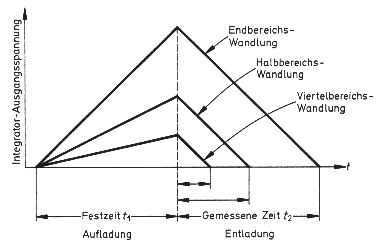
\includegraphics[width=8cm]{image/4/8}
\end{figure}

\paragraph{Beschreiben und erklären Sie die Funktionsweise eines Flash Analog-Digital Umsetzers.} ~

Flash-Umsetzer sind sogenannte Paralellumsetzer, bei denen alle logischen Entscheidungen parallel
ausgeführt werden. Sie zeichnen sich durch eine extrem schnelle Wandlungsgeschwindigkeit aus, die
nur einen Taktzyklus kurz ist.

Die Komperatoren haben zwei Eingänge, an welchen einerseits die Eingangsspannung verbunden ist und
am anderen über eine Widerstandsmatrix eine Bezugsspannung bezogen wird. Das analoge Eingangssignal
wird parallel an viele sogenannte Komparatoren geführt, wo es mit den erzeugten Referenzspannungen
verglichen wird. Hierbei ist für jeden möglichen Ausgangswert ein eigener Komparator erforderlich,
was bedeutet dass die Anzahl der Komparatoren exponentiell mit der Auflösung steigt.

Die Ausgänge der Komparatoren representieren diskrete digitale Zustände, deren Pegel codiert und
digitalisiert in jedem Taktzyklus als Ausgangssignal weitergeleitet wird.

\begin{figure}[H]
    \centering
    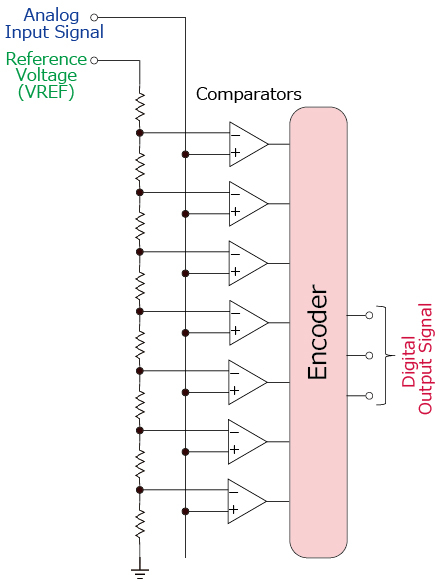
\includegraphics[height=6cm]{image/4/9}
\end{figure}

\paragraph{Aus welchen Beiträgen setzt sich die Gesamtunsicherheit eines Digitalvoltmeters
zusammen?} ~

\begin{itemize}
    \item Abgleichabweichung: Die Kennlinie eines Analog-Digital-Umsetzers ist eine Gerade durch den
        Nullpunkt und steht für die gewünschte Proportionalität zwischen Anzeige und Messgröße.
        Sowohl die horizontale Verschiebung zum Nullpunkt als auch die Steigung der Kennlinie können
        nur innerhalb gewisser Unsicherheitsgrenzen eingestellt werden.
    
    \item Quantisierungsabweichung: Dadurch, dass die Messgröße nur schrittweise abgebildet wird,
        entsteht eine Quantisierungsabweichung.
    
    \item Linearitätsabweichung: Man unterscheidet zwischen einer integralen Linearitätsabweichung
        durch eine Nichtlinearität der Kennlinie und einer differenziellen Linearitätsabweichung
        durch ungleiche Breite der benachbarten Quantisierungsschritte.
\end{itemize}

\paragraph{Die maximal messbare Spannung eines Voltmeters mit Innenwiderstand $R_i$ ist $U_m$. Der
Messbereich soll auf $10 \cdot U_m$ erweitert werden. Zeichnen und dimensionieren Sie eine
Widerstandsschaltung die dies ermöglicht. Wie groß ist der Gesamtwiderstand dieser Schaltung?} ~

Es muss zusätzlich ein Widerstand $R_V = 9 \cdot R_i$ in Serie vor das Voltmeter geschaltet werden.
Dies verzehnfacht den gesamten Innenwiderstand des Voltmeters, wobei aber $\frac{9}{10}$ am
Vorwiderstand abfallen. Damit sind auch 10 mal größere Messwiderstände möglich, was entsprechend
zum zehnfachen Messbereich für $U_m$ führt.

\begin{figure}[H]
    \centering
    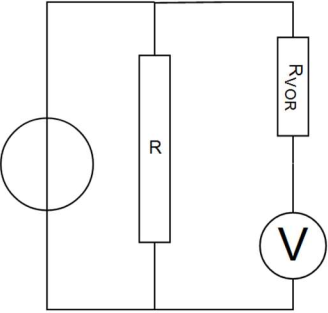
\includegraphics[height=4cm]{image/4/11}
\end{figure}

\paragraph{Die maximal mit einem Amperemeter (Innenwiderstand $R_i$) messbare Strom sei $I_m$. Der
Messbereich soll auf $10 \cdot I_m$ erweitert werden. Zeichnen und dimensionieren Sie eine
Widerstandsschaltung die dies ermöglicht. Wie groß ist der Gesamtwiderstand dieser Schaltung?} ~

Es muss zusätzlich ein Widerstand $R_m = \frac{R_i}{9}$ parallel zum Amperemeter geschaltet. Dadurch
wird der Strom vor das Amperemeter aufgeteilt, nur noch ein Zehntel fließt durch das Amperemeter.
Dies ermöglicht die Messung eines verzehnfachten Stromes.

\begin{figure}[H]
    \centering
    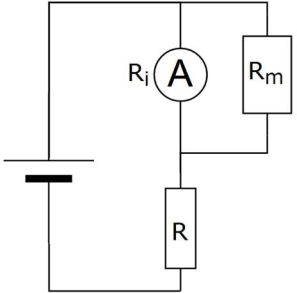
\includegraphics[height=4cm]{image/4/12}
\end{figure}

\newpage

\section{Statische Magnetfelder}

\paragraph{Schreiben Sie das Ampere‘sche Gesetz an. Leiten Sie daraus einen Ausdruck für das
Magnetfeld eines geraden, sehr langen, zylindrischen Leiters ab, durch den ein elektrischer Strom
mit über den Leiterquerschnitt homogener Stromdichte fließt.}
Das Ringintegral entlang einer geschlossenen Magnetfeldlinie, ist immer gleich dem eingeschlossenen Strom mal der magnetischen Feldkonstante,
wie aus dem Amperschen Gesetz \ref{AmperschesGesetz} ersichtlicht wird.  
\begin{equation} \\
    \oint \textbf{B} \hspace{0.2em} d\textbf{s} = \mu_0\cdot I
\end{equation}
Wählt man nun als Integrationsweg die den Draht umschließende Feldlinie mit dem Abstand $r$, so ergibt sich:
\begin{equation}
    \int_{0}^{2\pi} rBd\phi = 2 \pi r B(r) = \mu_0\cdot I
\end{equation}
\begin{equation}
    B(r) = \frac{\mu_0\cdot I}{2 \pi r} \hspace{2.5em} \text{für} \hspace{1em} r > r_0
\end{equation}
\begin{equation}
    B(r) = \frac{\mu_0\cdot I}{r_{0}^{2} 2 \pi} \cdot r  \hspace{2.5em} \text{für} \hspace{1em} r < r_0
\end{equation}
\paragraph{Schreiben Sie das Ampere‘sche Gesetz an. Leiten Sie daraus einen Ausdruck für das
Magnetfeld im Inneren einer geraden, sehr langen, zylindrischen Leiterspule ab.} 
Der Integrationsweg wird so gewählt, dass nur der Teil im Inneren der Spule einen Beitrag leistet.
\begin{figure}[H]
    \centering
    \label{Integrationsweg}
    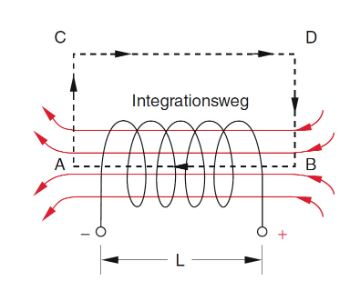
\includegraphics[height=7cm]{image/5/5.2.JPG}
\end{figure}
$N$ ist in diesem Zusammenhang die Anzahl der Windungen.
\begin{equation}
    \int_A^{B} B \hspace{0.2em} ds = B\cdot L = N\mu_0 I
\end{equation}
\begin{equation}
    B = \frac{N}{L}\mu_0 I \hspace{5em} \text{mit} \hspace{1em} \frac{N}{L} = n \hspace{0.5em} \text{(Windungsdichte)}
\end{equation}
\paragraph{Schreiben Sie einen Ausdruck für die Lorentzkraft (nicht die verallgemeinerte
Lorentzkraft) einer bewegten Ladung im Magnetfeld an. Beschreiben Sie alle verwendeten Formelsymbole
und leiten Sie damit die Kraft auf einen geraden, stromdruchflossenen Leiter im homogenen Magnetfeld
her.}
\begin{equation}
    \textbf{F} = q(\textbf{v} \times \textbf{B})
\end{equation}
\begin{itemize}
    \item $q$ Ladung auf die die Kraft wirkt 
    \item \textbf{v} die Geschwindigkeit des Ladungsträgers
    \item \textbf{B} Magnetfeld, welches der Ladungsträgert passiert
\end{itemize}
\begin{equation}
    d\textbf{F} = (\textbf{j} \times \textbf{B})\hspace{0.2em} dV \hspace{3em} dV = A\cdot dL \hspace{1em}\& \hspace{1em} j \cdot A = I
\end{equation}
\begin{align}
    d\textbf{F} &= I (d\textbf{L} \times \textbf{B})  \\
    \notag \\ 
    \textbf{F} &= I (\textbf{L} \times \textbf{B})
\end{align}
\paragraph{Schreiben Sie eine Ausdruck für das Magnetfeld zweier paralleler, stromdurchflossener,
zylindrischer Leiter an. Erstellen Sie ein Diagramm der magnetischen Feldstärke als Funktion des
Ortes entlang einer Linie, die die Achsen beider Leiter unter \SI{90}{\degree} schneidet. Welche
Richtung hat das Magnetfeld entlang dieser Linie?} 
\vspace{1em}
Das Magnetfeld des einen Leiters übt eine Kraft, abhängig von der Stromrichtung, auf den anderen aus.
Dieses Magnetfeld  $B = \frac{\mu_0 I}{2 \pi r} \cdot \hat{e}^{\phi}$ steht tangential auf konzentrischen Feldlinien.
Setzt man diesen Zusammenhang in die hergeleitete Formel der letzten Frage, so bemerkt man das $B$ orthognal auf $L$ steht, falls die zwei Drähte parallel zu einander verlaufen. 
Somit ergibt sich:
\begin{align}
    F_1 &= I_1(L_1 \cdot \frac{\mu_0 I_2}{2 \pi r} ) \\
    \\
    \frac{F_1}{L_1} &= \frac{\mu_0}{2 \pi r} \cdot I_2 \cdot I_1
\end{align}
\newpage
\paragraph{Leiten Sie ausgehend von der Kraft auf einen stromdurchflossenen, geraden Draht im
homogenen Magnetfeld einen Ausdruck für das Drehmoment einer rechteckigen Leiterschleife im
homogenen Magnetfeld her. Die Drehachse ist parallel zu zwei Seiten der Leiterschleife und senkrecht
zur Richtung des Magnetfeldes. Bei welchem Winkel zwischen Leiterschleife und Magnetfeldrichtung ist
das Drehmoment maximal? Bei welchem Winkel ist der magnetische Fluss durch die Leiterschleife
maximal?}
\begin{figure}[H]
    \centering
    \label{Drehmoment}
    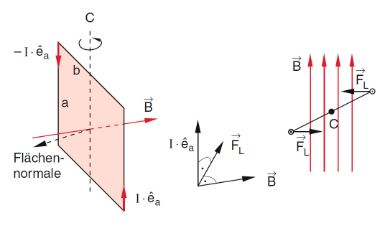
\includegraphics[height=6cm]{image/5/5.5.JPG}
\end{figure}
Ausgehend von den früher hergeleiteten Zusammenhang, kann man die Kraft, die auf die Leiterschleife wirkt als das Kreuzprodukt zwischen der Seite $a$ und dem Magnetfeld $B$ interpretieren. 
Diese wirkt nur auf die Längen $a$, da diese parallel zur Drehachse liegen und somit die Vektoren des Magnetfeldes in beiden Drähten entgegengestetzte Richtungen aufzeigen.
\begin{equation}
    F = a I ( \hat{e}_a \times B)
\end{equation}
Um das wirkende Drehmoment zu bestimmen, wird das Kreuzprodukt des Abstandes vom Drehmittelpunkt mit der auf die Teile der Leiterschleife wirkende Kraft gebildet.
\begin{equation}
    \textbf{M} = 2\frac{b}{2} ( \hat{e}_b \times \textbf{F}) = abl (\hat{e}_b \times \hat{e}_a) \times \textbf{B} = I(\textbf{A}\times\textbf{B})
\end{equation}
Was man aus diesem Zusammenhang erkennt ist, dass das Drehmoment am größten ist wenn der Flächennormalvektor $\textbf{A}$ orthogonal und somit im 90° Winkel zum Vektorfeld $\textbf{B}$ steht
\paragraph{Ein geladenes Teilchen ist bei $t=0$ am Ort $x=(0,0,0)$ mit der Geschwindigkeit
$v=(v_x,0,v_z)$ in einem homogenen Magnetfeld $B=(0,0,B_z)$. Wie wird die weitere Bahn des Teilchens
qualitativ aussehen und warum? Berechnen Sie die Kreisfrequenz und Radius.}
Das Teilchen beschreibt eine Spiralförmige Bahn, da aus der Lorenzkraft folgt, dass die auf das Teilechen wirkende Kraft sich zu $F = q(\textbf{v} \times \textbf{B})$ ergibt.
Hierzu ist nur die $v_x$ komponente entscheidend, was sich trivialerweise aus dem Kreuzprodukt ergibt. Um auf den Radius $R$ und die Kreisfrequenz $\omega$ schließen zu können setzt man die Lorenzkraft mit der Zentrifugalkraft gleich. 
\begin{figure}[H]
    \centering
    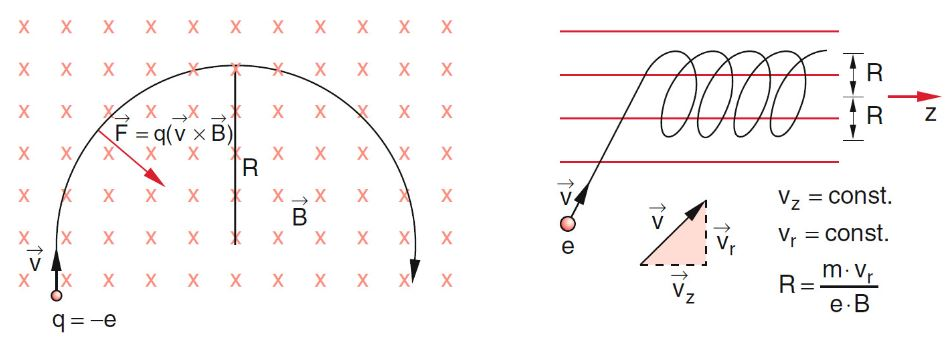
\includegraphics[height=5.5cm]{image/5/5.6.JPG}
\end{figure}
\begin{align}
    R &= \frac{mv_x}{qB} \\ 
    \\
    \omega &= \frac{v}{R} = \frac{q}{m} B
\end{align}
\paragraph{Beschreiben Sie die Funktion und Aufbau eines Wien-Filters und leiten Sie einen Ausdruck
für die Filter-Geschwindigkeit her.} 
Teilchen in einem Geschwindigkeitsintervall werden nicht bzw. wenig abgelenkt. Durch das Varieren des E-feldes und B-Feldes wird die gewünschte
Geschwindigkeit angepasst. Das Intervall kann direkt mit der Änderung der Spaltenbreite $\varDelta b$ und der Weglänge $\varDelta l$ skaliert werden.
\begin{figure}[H]
    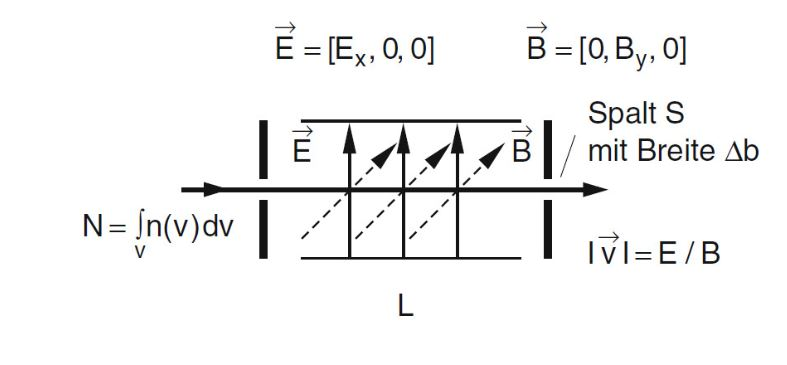
\includegraphics{image/5/5.7.JPG}
\end{figure}
\begin{align}
    \textbf{F} &= q(\textbf{E} + \textbf{v} \times \textbf{B}) = 0 \\
    \\
    v &= \frac{E}{B}
\end{align}
\paragraph{Beschreiben Sie den Hall-Effekt und leiten Sie ausgehend von der Lorentzkraft einen
Ausdruck für die Hall-Spannung für einen Leiter mit rechteckigem Querschnitt im homogenen Magnetfeld
her.} 
Bewegt sich ein Ladungsträger durch ein homogenes Magnetfeld, so wird er senktrecht dazu abgelenkt. Diese Ablenkung führt zu einer inhomogenen Ladungsverteilung im Medium und zu einer Ansammlung der Ladungströger an den Äquipotenzialflächen.
Diese wiederum tragen zu einem sich aufbauenden E-Feld bei. Durch Variation der Stromstärke wird die Stärke des E-Feldes beeinflusst, die durch dieses E-Feld erzeugte Kraft, die der Lorenzkraft engegenwirkt, und der an den Aquipotenzialflächen abgreifbare Spannung $U_H$ (Hallspannung).
\begin{figure}[H]
    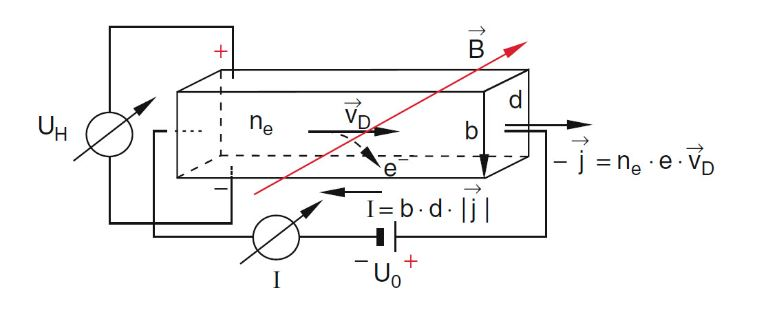
\includegraphics{image/5/5.8.JPG}
\end{figure}
\begin{align}
   \textbf{F}_B &= nq(\textbf{v}_D \times \textbf{B}) \\
  \\
   \textbf{F}_E &= nq \textbf{E}_H\\
   \\
   nq \textbf{E}_H &= -qn(\textbf{v}_D \times \textbf{B}) \hspace{5em} U_H = \int \textbf{E}_H d\textbf{s} = \textbf{E}_H \cdot \textbf{b} \\
   \\
   U_H &= - \frac{(\textbf{j} \times \textbf{B})\cdot b} {nq}      \hspace{5em} I = \textbf{j}\cdot \textbf{A} = j\cdot b \cdot d \\
   \\
   U_H &= -\frac{I\cdot B}{nqd}
\end{align}

\paragraph{Wie beeinflussen Stromdichte, Querschnittsabmessungen, Ladungsträgerdichte und Ladung
der Ladungsträger die Hall-Spannung? Geben Sie an, ob die Parameter groß oder klein sein sollten, um
eine möglichst große Hall-Spannung zu beobachten.}
Die Dicke $d$, die Ladungsträgerdichte $n$ und Ladung $q$ sollten möglichst klein und die Stromstärke $I$ , das stationäre Magnetfeld $B$
sollten möglichst groß sein, um eine große Hall-Spannung zu erzeugen. Die Ladungsträgerdichte ist eine spezifiche Größe für jedes Material, genauso sowie die Ladung selbst, was zufolge hat, dass
bei gleicher Stromstärke verschiedene Stoffe unterschieldliche Driftgeschwindigkeiten besitzen. Je größer die Driftgeschwindigkeit, desto größer ist die wirkende Lorenzkraft.
Die Querschnittsabmessungen beinflussen die Spannung massiv, für große Hallspannungen sollte hierzu $b$ größer gewählt werden.

\newpage

\section{Materie im magnetischen Feld}

\paragraph{Ein kleiner Probekörper mit bekanntem Volumen befindet sich in einem inhomogenen
magnetischen Feld. Der Probekörper wird durch das äußere Magnetfeld magnetisiert und erfährt daher
eine Kraft. Wie groß ist diese Kraft und welche Richtung hat sie bei positiver oder negativer
magnetischer Suzeptiblität?} ~

\begin{equation}
    \bold{F} = \bold{p_m} \cdot \nabla \bold{B} = - M \cdot V \cdot \frac{dB}{dr} \bold{\hat{r}}
\end{equation}

Für die Magnetisierung $M = \chi \cdot H$ ergibt sich bei diamagnetischen Stoffen ($\chi < 0$) eine
radiale Kraft nach außen, paramagnetische Stoffe ($\chi > 0$) hingegen werden zum Zentrum gezogen.

\begin{figure}[H]
    \centering
    \begin{minipage}[b]{0.3\textwidth}
        \centering
        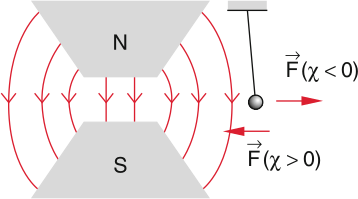
\includegraphics[height=3cm]{image/6/1.1}
    \end{minipage}
    \hspace{2cm}
    \begin{minipage}[b]{0.3\textwidth}
        \centering
        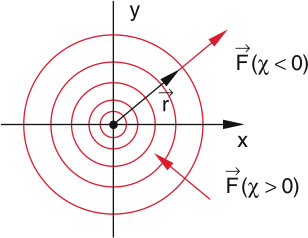
\includegraphics[height=3cm]{image/6/1.2}
    \end{minipage}
\end{figure}

\paragraph{Welche magnetischen Stoffklassen gibt es und wie unterscheiden sie sich in ihren
magnetischen Eigenschaften?} ~

\begin{itemize}
    \item Konstante magnetische Suszeptibilität $\chi$
    
        \begin{itemize}
            \item \textbf{Paramagnete} besitzen ein permanentes magnetisches Dipolmoment
                $\bold{p_m}$, welches aber aufgrund thermischer Bewegung statistisch im Raum 
                verteilt ist und in Summe Null ergibt.
                
                Durch ein äußeres Magnetfeld werden die Dipole parallel ausgerichtet und verstärken
                so das äußere Feld im Inneren des Stoffes. Mit steigender Temperatur sinkt die
                Suszeptibilität.
                
                Paramagnete werden im inhomogenen Magnetfeld zur höheren Feldstärke hingezogen.
                
            \item \textbf{Diamagnete} besitzen kein eigenes magnatisches Dipolmoment $\bold{p_m}$.
                Sie entwickeln im  äußeren Magnetfeld ein induziertes, inneres Magnetfeld, welches
                dem äußeren entgegenwirkt.
                
                Diamagnete werden im inhomogenen Magnetfeld zur niederen Feldstärke hingezogen.
        \end{itemize}
    
    \item Variable magnetische Suszeptibilität $\chi$
        
        \begin{itemize}
            \item \textbf{Ferromagnete} besitzen eine hohe magnetische Suszeptibilität $\chi$, die
                Magnetisierung $M$ kann im Vergleich zu Paramagneten um viele Größenordnungen höher
                sein.
                
                Sie richten im externen Feld ihre magnetischen Momente innerhalb kleiner Bereiche
                (Weiß'sche Bezirke) parallel aus und behalten diese Ausrichtung auch nach Entfernung
                des Feldes. Ferromagnete erzeugen entweder selbst ein dauerhaftes Magnetfeld oder
                werden von einem Pol eines äußeren Magnetfelds stark angezogen.
                
                Über der sogenannten Curie-Temperatur wird die magnetische Ordnung aufgebrochen,
                der Stoff ist dann nur noch paramagnetisch.
                
                \begin{figure}[H]
                    \centering
                    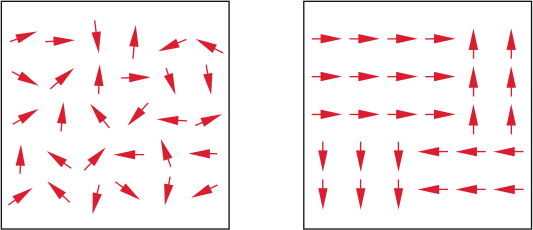
\includegraphics[height=3cm]{image/6/2.1}
                \end{figure}
            
            \item \textbf{Antiferromagnete} weisen ein Kristallgitter mit zwei ineinander gestellten
                Untergittern auf, wobei ohne äußeres Magnetfeld die magnetischen Momente der Atome
                A des einen Gitters antiparallel zu denen der Atome B im anderen Gitter stehen,
                wodurch die Magnetisierung $M$ insgesamt Null ist.
                
                Ähnlich wie bei Ferromagneten gehen die Antiferromagnete bei der kritischen,
                sogenannten Néel-Temperatur in den paramagnetischen Zustand über.
                
                \begin{figure}[H]
                    \centering
                    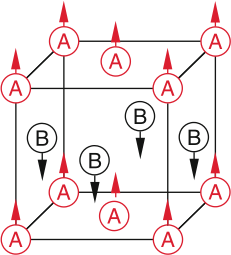
\includegraphics[height=3cm]{image/6/2.2}
                \end{figure}
            
            \item \textbf{Ferrimagnete} weisen wie Antiferromagnete zwei Untergitter auf, allerdings
                sind die magnetischen Momente der verschiedenen Atome unterschiedlich groß, sodass
                sich eine spontane Magnetisierung auch ohne äußeres Feld ergibt.
                
                Sie weisen eine ähnliche Magnetisierungskurve wie Ferromagnete auf, die
                Sättigungsmagnetisierung ist allerdings wesentlich geringer.
        \end{itemize}
\end{itemize}

\paragraph{Was versteht man unter Diamagnetismus und Paramagnetismus? Welche spezielle Eigenschaft
haben Moleküle oder Atome eines dia- oder paramegnetischen Stoffes?} ~

\begin{itemize}
    \item \textbf{Paramagnete} besitzen ein permanentes magnetisches Dipolmoment
        $\bold{p_m}$, welches aber aufgrund thermischer Bewegung statistisch im Raum 
        vererteilt ist und in Summe Null ergibt.
        
        Durch ein äußeres Magnetfeld werden die Dipole parallel ausgerichtet und verstärken
        so das äußere Feld im Inneren des Stoffes. Mit steigender Temperatur sinkt die
        Suszeptibilität.
        
        Paramegnete werden im inhomogenen Magnetfeld zur höheren Feldstärke hingezogen.
        
    \item \textbf{Diamagnete} besitzen kein eigenes magnatisches Dipolmoment $\bold{p_m}$.
        Sie entwickeln im  äußeren Magnetfeld ein induziertes, inneres Magnetfeld, welches
        dem äußeren entgegenwirkt.
        
        Diamagnete werden im inhomogenen Magnetfeld zur niederen Feldstärke hingezogen.
\end{itemize}

\paragraph{Beschreiben Sie die Eigenschaften eines ferromagnetischen Stoffes? Nennen Sie drei
Beispiele für ferromagnetische Stoffe.} ~

Ferromagnetismus tritt nur in Festkörpern auf. Ferromagnete zeigen die Tendenz, ihre magnetische
Ordnung auch entgegen äußeren Einflüssen zu behalten. Dies führt dazu, dass die im Inneren erzeugte
magnetische Ordnung und somit das äußere erzeugte Magnetfeld behalten, auch wenn sie keinem
Magnetfeld mehr ausgesetzt sind. Diese als Remanenz bezeichnete Tendenz wird durch Effekte in zwei
verschiedenen Größenordnungen verursacht:

\begin{itemize}
    \item Mikroskopisch: Die gleichgerichtete magnetische Ordnung der Elementarmagnete (also
        beispielsweise der Elektronenspins) in atomarer Größenordnung.
        
    \item Makroskopisch: Die Anordnung der Weiß-Bezirke in der Größenordnung von Mikro- bis
        Nanometern.
\end{itemize}

Die meisten ferromagnetischen Materialien bestehen aus Übergangselementen, also aus Atomen mit nicht
aufgefüllten inneren Elektronenschalen wie Eisen, Nickel oder Kobalt. Über der sogenannten
Curie-Temperatur wird die magnetische Ordnung aufgebrochen, der Stoff ist dann nur noch
paramagnetisch.

\paragraph{Was sind antiferromagnetische und ferrimagnetische Stoffe?} ~

\begin{itemize}
        \item \textbf{Antiferromagnete} weisen ein Kristallgitter mit zwei ineinander gestellten
            Untergittern auf, wobei ohne äußeres Magnetfeld die magnetischen Momente der Atome
            A des einen Gitters antiparallel zu denen der Atome B im anderen Gitter stehen,
            wodurch die Magnetisierung $M$ insgesamt Null ist.
            
            Ähnlich wie bei Ferromagneten gehen die Antiferromagnete bei der kritischen,
            sogenannten Néel-Temperatur in den paramagnetischen Zustand über.
            
            \begin{figure}[H]
                \centering
                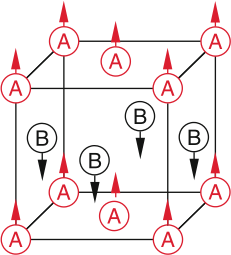
\includegraphics[height=3cm]{image/6/2.2}
            \end{figure}
        
        \item \textbf{Ferrimagnete} weisen wie Antiferromagnete zwei Untergitter auf, allerdings
            sind die magnetischen Momente der verschiedenen Atome unterschiedlich groß, sodass
            sich eine spontane Magnetisierung auch ohne äußeres Feld ergibt.
            
            Sie weisen eine ähnliche Magnetisierungskurve wie Ferromagnete auf, die
            Sättigungsmagnetisierung ist allerdings wesentlich geringer.
    \end{itemize}

\paragraph{Schreiben Sie die Feldgleichungen der Elektro- und Magnetostatik an. Welche
Stetigkeitsbedingungen müssen die elektrischen und magnetischen Felder an Grenzflächen erfüllen?} ~

\begin{itemize}
    \item \textbf{Elektrostatik:} Mit den Stetigkeitsbedingungen $E_{\parallel,1} = E_{\parallel,2}$
        sowie $D_{\perp,1} = D_{\perp,2}$ gilt
        
        \begin{equation}
            \bold{D} = \epsilon_0 \epsilon \bold{E}
        \end{equation}
        \begin{equation}
            \oint \bold{D} d\bold{A} = Q ~~~ \text{bzw} ~~~ div~\bold{D} = \rho
        \end{equation}
        \begin{equation}
            \oint \bold{E} d\bold{s} = 0 ~~~ \text{bzw} ~~~ rot~\bold{E} = 0
        \end{equation}
        
    \item \textbf{Magnetostatik:} Mit den Stetigkeitsbedingungen $H_{\parallel,1} = H_{\parallel,2}$
        sowie $B_{\perp,1} = B_{\perp,2}$ gilt
        
        \begin{equation}
            \bold{B} = \mu_0 \mu \bold{H}
        \end{equation}
        \begin{equation}
            \oint \bold{B} d\bold{A} = 0 ~~~ \text{bzw} ~~~ div~\bold{B} = 0
        \end{equation}
        \begin{equation}
            \oint \bold{H} d\bold{s} = I_A ~~~ \text{bzw} ~~~ rot~\bold{H} = \bold{j}
        \end{equation}
\end{itemize}

\newpage

\section{Zeitlich veränderliche Felder}

\paragraph{Schreiben Sie das Faradaysche Induktionsgesetz an. Welche Prozesse können zu einer
induzierten Spannung in einer Leiterschleife führen?} ~

\begin{equation}
    U_{ind} = - \frac{d}{dt} \int \bold{B} d\bold{A} = - \frac{d \phi_m}{dt}
\end{equation}

Eine induzierte Spannung kann durch Änderung der magnetischen Feldstärke $\bold{B}$, des
Flächeninhalts $A$ oder der Orientierung der beiden Größen relativ zueinander hervorgerufen werden.

\paragraph{Eine quadratische Leiterschleife (Schleifenfläche A) dreht sich im homogenen Magnetfeld
mit der Winkelgeschwindigkeit $\omega$ um eine Achse, die senkrecht zu den magnetischen Feldlininen
steht. Schreiben Sie einen Ausdruck für die induzierte Spannung als Funktion des Winkels und der
Zeit an. Bei welcher Orientierung der Leiterschleife relativ zum Magnetfeld ist die induzierte
Spannung maximal (Skizze!)?} ~

\begin{equation}
    \phi_m = \int \bold{B} d\bold{A} = B \cdot A \cdot cos(\omega \cdot t)
\end{equation}
\begin{equation}
    U_{ind} = - \frac{d}{dt} \phi_m = B \cdot A \cdot \omega \cdot sin(\omega \cdot t)
\end{equation}

\begin{figure}[H]
    \centering
    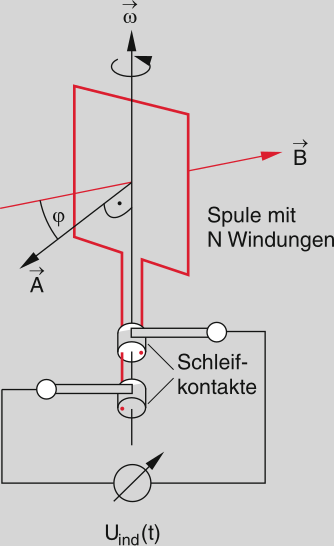
\includegraphics[height=6cm]{image/7/2.1}
\end{figure}

Die induzierte Spannung ist maximal, wenn die Flächennormale mit $\varphi = \SI{90}{\degree}$
senkrecht auf das Magnetfeld steht.

\paragraph{Eine offene Leiterschleife befindet sich in einem homogenen Magnetfeld. Der
Flächennormalvektor steht parallel zu den Feldlinien. Die magnetische Feldstärke nimmt mit der Zeit
zu. Skizzieren Sie die Situation und zeichnen Sie die Richtung der induzierten elektrischen
Feldstärke sowie die Polarität der beiden offenen Enden der Leiterschleife ein.} ~

\begin{figure}[H]
    \centering
    \begin{minipage}[b]{0.3\textwidth}
        \centering
        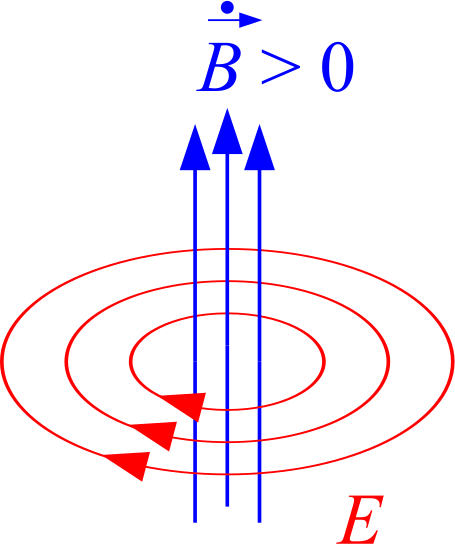
\includegraphics[height=3cm]{image/7/3.1}
    \end{minipage}
    \hspace{2cm}
    \begin{minipage}[b]{0.3\textwidth}
        \centering
        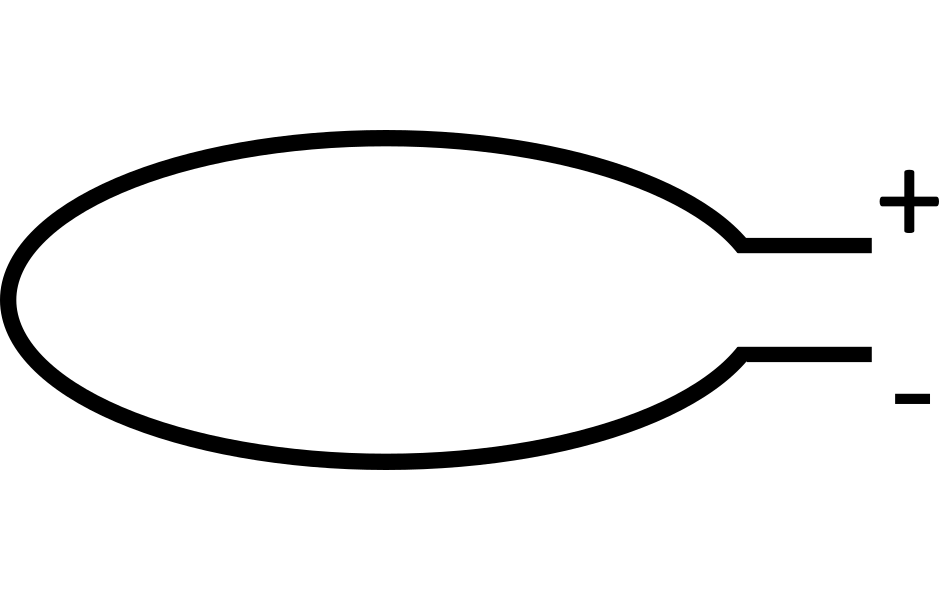
\includegraphics[height=3cm]{image/7/3.2}
    \end{minipage}
\end{figure}

\paragraph{Beschreiben Sie Aufbau und Funktion einer Induktionsschleuder.} ~

Auf einem langen Eisenjoch liegt über einer Feldspule ein Aluminiumring. Wird die Spule
eingeschaltet, so wird im Ring ein Induktionsstrom erzeugt dessen magnetisches Moment so gerichtet
ist, dass der Ring hochgeschleudert wird. Dieses Prinzip kann technisch angewandt werden, um
kleinere Projektile auf große Geschwindigkeiten von bis zu \SI{8}{\km\per\s} beschleunigen.

\begin{figure}[H]
    \centering
    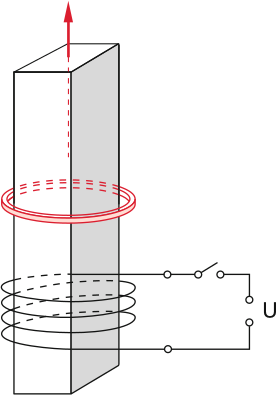
\includegraphics[height=5cm]{image/7/4}
\end{figure}

\paragraph{Was versteht man unter Selbstinduktion? Was bedeutet der Selbstinduktionskoeffizient?} ~

In einer stromdurchflossenen Spule wird bei einer zeitlichen Änderung des Stromes der magnetische
Fluss durch die Spule geändert, weshalb nun aufgrund des Magnetfelds der Spule auch in der Spule
selbst eine Induktionsspannung entsteht. Diese ist gemäß der Lenz'schen Regel der Änderung der von
außen angelegten stromtreibenden Spannung entgegengerichtet.

Da das von der Spule erzeugte Magnetfeld proportional zum Strom $I$ durch die Spule ist, folgt mit
$\phi_m = L \cdot I$ die Proportionalitätskonstante $L$ mit der Maßeinheit Henry, welche auch als
Selbstinduktionskoeffizient bekannt ist.

\paragraph{Eine Doppelleitung besteht aus zwei zylindrischen, parallelen Leitern, durch die der
gleiche Strom aber mit unterschiedlichen Vorzeichen fließt. Fertigen Sie eine Skizze an, skizzieren
Sie das Magnetfeld der Anordnung und schreiben Sie das Magnetfeld zwischen den Leitern analytisch
an. Zeigen Sie, wie man daraus (im Prinzip) den Selbstinduktionskoeffizienten der Doppelleitung
berechnen kann.} ~

\begin{equation}
    B_a = \frac{\mu_0 I}{2 \pi} \left( \frac{1}{\frac{d}{2} + x} + \frac{1}{\frac{d}{2} - x} \right)
\end{equation}
\begin{equation}
    B_{1i} = \frac{\mu_0 I}{2 \pi r_0^2} \left( \frac{d}{2} + x \right) + B_{2a}
\end{equation}
\begin{equation}
    B_{2i} = \frac{\mu_0 I}{2 \pi r_0^2} \left( \frac{d}{2} - x \right) + B_{1a}
\end{equation}
Durch Integration über die magnetische Flussdichte $B$ ergibt sich zunächst der magnetische Fluss
$\phi_m$ und in weiterer Folge der Selbstinduktionskoeffizient $L$.
\begin{equation}
    \phi_m = l \cdot \int_{-d/2}^{d/2} B dx
\end{equation}
\begin{equation}
    L
    = \frac{\phi_m}{I}
    = ...
    = \frac{\mu_0 I}{2 \pi} \left( 1 + 2 \cdot ln \frac{d - r_0}{r_0} \right)
\end{equation}

\begin{figure}[H]
    \centering
    \begin{minipage}[b]{0.3\textwidth}
        \centering
        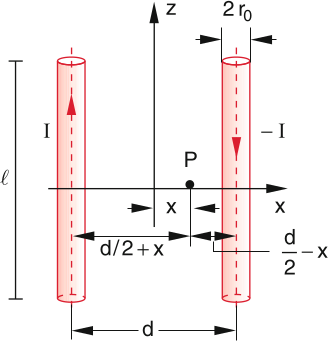
\includegraphics[height=4cm]{image/7/6.1}
    \end{minipage}
    \hspace{2cm}
    \begin{minipage}[b]{0.3\textwidth}
        \centering
        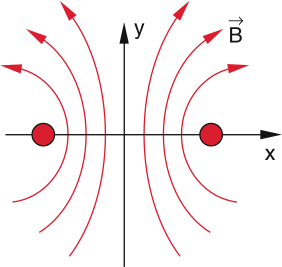
\includegraphics[height=4cm]{image/7/6.2}
    \end{minipage}
\end{figure}

\paragraph{Was versteht man unter Gegeninduktion? Wie kann man sie formal beschreiben?} ~

Ein vom Strom $I_1$ durchflossener Stromkreis 1 erzeugt im Punkt $\bold{P(r_2)}$ ein Magnetfeld
$\bold{B}$. Dieses Magnetfeld erzeugt einen magnetischen Fluss durch die vom Leiterkreis 2
eingeschlossene Fläche $A$. Die diesen Fluss $\phi_m = L_{12} \cdot I_1$ mit dem Strom $I_1$ im
Stromkreis 1 verknüpfende Proportionalitätskonstante $L_{12} = L_{21}$ heißt Koeffizient der
gegenseitigen Induktivität.

\begin{figure}[H]
    \centering
    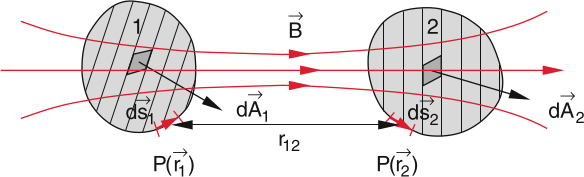
\includegraphics[width=8cm]{image/7/7}
\end{figure}

\paragraph{Beschreiben Sie den Strom- und Spannungsverlauf einer Serienschaltung aus idealer
Induktivität und ohm‘schen Widerstand, wenn diese über einen Schalter mit einer idealen
Spannungsquelle verbunden werden (Einschaltvorgang). Schreiben Sie die Funktionen $I(t)$ sowie
$U(t)$ für Widerstand und Spule an und erstellen Sie die entsprechenden Diagramme.} ~

\begin{equation}
    I(t) = \frac{U_0}{R} \cdot \left( 1 - e^{-Rt/L} \right)
\end{equation}
\begin{equation}
    U_L(t) = U_0 \cdot e^{-Rt/L} ~~~ U_R = U_0 \cdot \left( 1 - e^{-Rt/L}) \right)
\end{equation}

\begin{figure}[H]
    \centering
    \includegraphics[width=12cm]{image/7/8}
\end{figure}

\paragraph{Beschreiben Sie den Strom- und Spannungsverlauf einer Serienschaltung aus idealer
Induktivität und ohm‘schen Widerstand, wenn diese über einen Schalter von einer
Spannungsquelle plötzlich getrennt werden (Ausschaltvorgang). Schreiben Sie die
Funktionen $I(t)$ sowie $U(t)$ für Widerstand und Spule an und erstellen Sie die entsprechenden
Diagramme.} ~

\begin{equation}
    I(t) = \frac{U_0}{R} \cdot e^{-Rt/L}
\end{equation}
\begin{equation}
    U_L(t) = - U_0 \cdot e^{-Rt/L} ~~~ U_R = U_0 \cdot e^{-Rt/L}
\end{equation}

\begin{figure}[H]
    \centering
    \includegraphics[width=12cm]{image/7/9}
\end{figure}

\paragraph{Wie kann man im Prinzip die Induktivität z.B. einer Spule durch eine Zeitmessung
bestimmen (Schaltplan und Beschreibung)?} ~

Nach Anlegen einer Gleichspannung und Schließen des Schalters kann die Zeitverzögerung
$\tau = \frac{L}{R}$ zwischen dem Aufleuchten der Lampen gemessen werden. Aus diesem Zusammenhang
folgt die Induktivität $L$, wenn der ohm'sche Widerstand der Spule bekannt ist.

Dieser lässt sich durch gleichzeitiges Messen der abfallenden Spannung an der Spule sowie des zu
diesem Zeitpunkt fließenden Stroms mit $R = \frac{U}{I}$ ermitteln.

\begin{figure}[H]
    \centering
    \includegraphics[width=5cm]{image/7/10}
\end{figure}

\paragraph{Zwei dünne, lange Spulen sind auf den gleichen Kern gewickelt, sodass der gesamte
magnetische Fluss der einen Spule durch die andere fließt. Berechnen Sie die in einer Spule
induzierte Spannung, wenn sich in der andern der Strom ändert. Die Spulenlängen, die Anzahl der
Windungen, die Spulenquerschnitte, und die magnetischen Eigenschaften des Spulenkerns seien
bekannt.} ~

\begin{equation}
    U_{ind} = -L \cdot \dot{I}
    = - \mu_r \mu_0 n^2 \frac{A}{l} \cdot \dot{I}
\end{equation}

\paragraph{Berechnen Sie die im magnetischen Feld einer dünnen, langen Spule gespeicherte Energie
als Funktion des Stromes. Die Spulenlänge, die Anzahl der Windungen, der Spulenquerschnitt, und die
magnetischen Eigenschaften des Spulenkerns seien bekannt.}

\begin{equation}
    W(I) = \frac{1}{2} \cdot I^2 \cdot L = \frac{1}{2} \cdot I^2 \cdot \mu_r \mu_0 n^2 \frac{A}{l}
\end{equation}

\paragraph{Schreiben Sie die Maxwell-Gleichungen an und visualisieren Sie die Quellen der
elektrischen und magnetischen Felder sowie die Ursache der elektrischen und magnetischen
Wirbelfelder. (vgl. Folie 23).} ~

\begin{equation}
    rot~\bold{E} + \pdv{\bold{B}}{t} = 0 ~~~ div~\bold{D} = \rho
\end{equation}
\begin{equation}
    rot~\bold{H} - \pdv{\bold{D}}{t} = \bold{j} ~~~ div~\bold{B} = 0
\end{equation}

\begin{figure}[H]
    \centering
    \includegraphics[width=8cm]{image/7/13}
\end{figure}

\newpage

\section{Elektrische Generatoren und Motoren}

\paragraph{Erklären Sie das Prinzip eines einfachen Wechselstromgenerators mit einer Spule im
homogenen äußeren Magentfeld. Schreiben Sie die Beziehung für den elektrischen Fluss an und leiten
Sie daraus die induzierte Spannung bei konstanter Winkelgeschwindigkeit als Funktion der Zeit
her.} ~

Eine rechteckige Spule mit der Windungsfläche $A$ befindet sich im homogenen Magnetfeld $\bold{B}$
und wird mit der Winkelgeschwindigkeit $\omega$ gedreht. Dabei wird an den Enden der Spule eine
Wechselspannung induziert, welche über zwei Schleifkontakte abgegriffen werden kann.

\begin{figure}[H]
    \centering
    \includegraphics[width=7cm]{image/8/1}
\end{figure}

\begin{equation}
    \phi_m = \int \bold{B} d\bold{A} = B \cdot A \cdot cos(\omega \cdot t)
\end{equation}
\begin{equation}
    U_{ind} = - \frac{d}{dt} \phi_m = B \cdot A \cdot \omega \cdot sin(\omega \cdot t)
\end{equation}

\paragraph{Doppel-T Anker und Trommelanker: Beschreiben Sie die Funktion eines permanenterregten
Generators mit Doppel-T Anker und Kommutator. Skizzieren Sie den Anker inklusive Stellung und
Anschluss des Kommutators relativ zur Spulenorientierung. Erstellen Sie ein Diagramm der
Klemmspannung als Funktion der Zeit für konstante Drehgeschwindigkeit. Welche Vorteile bringt ein
Trommelanker?} ~

Am permanent erregten Generator wird das magnetische Feld durch einen als Stator dienenden
Permanentmagneten erzeugt. Die bei Drehung des Rotors in den Spulen induzierte Spannung wird über
den Kommutator abgenommen, welcher je nach Anzahl der Spulen unterschiedlich viele Schleifkontakte
aufweist.

Die Verwendung eines Trommelankers stellt im Gegensatz zum Doppel-T-Anker eine Verbesserung dar,
bei der der magnetische Kraftfluss $\phi_m$ vergrößert wird. Mit der Anzahl der Spulen wird die
erzeugte Gleichspannung immer gleichmäßiger. Im Fall von Gleichstrommotoren ermöglicht ein
Trommelanker zudem ein selbständiges Anlaufen des Motors, da immer auf mindestens ein Ankerelement
ein Drehmoment wirkt.

\begin{figure}[H]
    \centering
    \begin{minipage}[b]{0.3\textwidth}
        \centering
        \includegraphics[width=3cm]{image/8/2.1}
    \end{minipage}
    \hspace{2cm}
    \begin{minipage}[b]{0.3\textwidth}
        \centering
        \includegraphics[width=6cm]{image/8/2.2}
    \end{minipage}
\end{figure}

\begin{figure}[H]
    \centering
    \includegraphics[height=7cm]{image/8/2.3}
\end{figure}

\paragraph{Skizzieren Sie den Aufbau und Schaltplan einer Hauptschlussmaschine. Wie sieht bei einem
Generator dieser Bauart die Klemmspannung als Funktion des Stromes aus? Wie sieht bei einem Motor
dieser Bauart der Strom und das Drehmoment als Funktion der Drehzahl bei konstanter
Versorgungsspannung aus?} ~

\begin{figure}[H]
    \centering
    \begin{minipage}[b]{0.3\textwidth}
        \centering
        \includegraphics[height=4cm]{image/8/3.1}
    \end{minipage}
    \hspace{2cm}
    \begin{minipage}[b]{0.3\textwidth}
        \centering
        \includegraphics[height=4cm]{image/8/3.2}
    \end{minipage}
\end{figure}

\begin{figure}[H]
    \centering
    \begin{minipage}[b]{0.3\textwidth}
        \centering
        \includegraphics[height=2cm]{image/8/3.3}
    \end{minipage}
    \hspace{2cm}
    \begin{minipage}[b]{0.3\textwidth}
        \centering
        \includegraphics[height=2cm]{image/8/3.4}
    \end{minipage}
\end{figure}

\paragraph{Skizzieren Sie den Aufbau und Schaltplan einer Nebenschlussmaschine. Wie sieht bei einem
Generator dieser Bauart die Klemmspannung als Funktion des Stromes aus? Wie sieht bei einem Motor
dieser Bauart der Strom und das Drehmoment als Funktion der Drehzahl bei konstanter
Versorgungsspannung aus?} ~

\begin{figure}[H]
    \centering
    \begin{minipage}[b]{0.3\textwidth}
        \centering
        \includegraphics[height=4cm]{image/8/4.1}
    \end{minipage}
    \hspace{2cm}
    \begin{minipage}[b]{0.3\textwidth}
        \centering
        \includegraphics[height=4cm]{image/8/4.2}
    \end{minipage}
\end{figure}

\begin{figure}[H]
    \centering
    \begin{minipage}[b]{0.3\textwidth}
        \centering
        \includegraphics[height=2cm]{image/8/4.3}
    \end{minipage}
    \hspace{2cm}
    \begin{minipage}[b]{0.3\textwidth}
        \centering
        \includegraphics[height=2cm]{image/8/4.4}
    \end{minipage}
\end{figure}

\paragraph{Nennen und erklären Sie drei Arten von Erregung bei Gleichstrommaschinen.} ~

\begin{itemize}
    \item Permanente Erregung: Das Statorfeld wird durch einen Permenentmagneten erzeugt.
    
    \item Elektrische Erregung: Das Statorfeld wird durch einen Elektromagneten erzeugt. Werden
        Erreger- und Ankerwicklung von der gleichen Quelle betrieben unterscheidet man je nach
        Schaltung zwischen einer Reihen- oder Nebenschlussmaschine. Bei unabhängigem Betrieb spricht
        man von Fremderregung.
\end{itemize}

\newpage

\section{Wechselstrom und Drehstrom}

\paragraph{Zeichnen Sie den zeitlichen Spannungsverlauf einer Wechselspannung. Zum Zeitpunkt $0$ sei
die Phase $\phi \neq 0$. Zeichnen Sie das Zeigerdiagramm für die Spannung zum Zeitpunkt $t=0$ und
$t=T/4$ , wobei $T$ die Periodendauer ist. Zeichnen Sie Periodendauer, Scheitelwert und Effektivwert
ein.} ~

\begin{figure}[H]
    \centering
    \includegraphics[width=10cm]{image/9/1}
\end{figure}

\paragraph{Eine Wechselspannungsquelle liefert an einen Verbraucher Spannung und Strom. Der Strom
eilt der Spannung um einen Phasenwinkel von \SI{45}{\degree} nach. Zeichnen Sie den zeitlichen
Spannungs- und Stromverlauf und das Zeigerdiagramm mit Spannung und Strom zum Zeitpunkt $t=0$ bei
dem die Spannung gerade ihr Maximum hat, und zum Zeitpunkt $t=T/4$, wobei $T$ die Periodendauer
ist.} ~

\begin{figure}[H]
    \centering
    \includegraphics[width=10cm]{image/9/2}
\end{figure}

\paragraph{Eine Wechselspannungsquelle liefert an einen Verbraucher Spannung und Strom. Der Strom
eilt der Spannung um einen Phasenwinkel von \SI{45}{\degree} voraus. Zeichnen Sie den zeitlichen
Spannungs- und Stromverlauf sowie den zeitlichen Verlauf der abgegebenen Leistung. Erklären und
berechnen Sie Wirk-, Blind-, und Scheinleistung.} ~

\begin{figure}[H]
    \centering
    \begin{minipage}[b]{0.3\textwidth}
        \centering
        \includegraphics[width=5cm]{image/9/3.1}
    \end{minipage}
    \hspace{2cm}
    \begin{minipage}[b]{0.3\textwidth}
        \centering
        \includegraphics[width=5cm]{image/9/3.2}
    \end{minipage}
\end{figure}

\begin{equation}
    \text{Scheinleistung:} ~~~ S = U \cdot I = \sqrt{P^2 + Q^2}
\end{equation}
\begin{equation}
    \text{Wirkleistung:} ~~~ P = S \cdot cos(\varphi)
\end{equation}
\begin{equation}
    \text{Blindleistung:} ~~~ Q = S \cdot sin(\varphi)
\end{equation}

\paragraph{Zeichnen Sie den zeitlichen Spannungsverlauf einer dreiphasigen Wechselspannung sowie das
zugehörige Zeigerdiagramm.} ~

\begin{figure}[H]
    \centering
    \includegraphics[width=10cm]{image/9/4}
\end{figure}

\paragraph{Zeichnen Sie die Schaltpläne für drei Widerstände, die in Stern- oder Dreieckschaltung an
eine dreiphasige Wechselspannung angeschlossen sind. Erstellen Sie die zugehörigen Zeigerdiagramme.
Berücksichitgen Sie im Zeigerdiagramm bei der Dreieckschaltung sowohl die Strangspannungen $U_i$ als
auch die Außenleiterspannungen $U_{ij}$ und deren Konstruktion.} ~

\begin{figure}[H]
    \centering
    \includegraphics[width=10cm]{image/9/5.1}
\end{figure}
Bei der Sternschaltung gilt in jedem Fall $I_1 + I_2 + I_3 + I_0 = 0$, bei symmetrischer Belastung
sogar $I_1 + I_2 + I_3= 0$.
\begin{figure}[H]
    \centering
    \includegraphics[width=10cm]{image/9/5.2}
\end{figure}
Bei der Dreieckschaltung gilt bei unsymmetrischer Belastung $I_1 + I_2 + I_3 \neq 0$.

\paragraph{Beschreiben und erklären Sie den Aufbau eines Asynchron-Motors mit Kurzschluss-Läufer.
(Skizze und Benennung aller wesentlicher Bauteile)} ~

Ist eine Drehstrommaschine, bei der der Rotor dem Drehfeld des Stators als Generator vor und als
Elektromotor nachläuft. Entweder strändig oder fallweise kurzgeschlossen. Dreht sich der Rotor
langsamer als das Magnetfeld ändert sich dadurch der magnetische Fluss, was eine Spannung induziert,
die wiederum einen Strom hervorruft. Fließt Strom durch die Ständerwicklung wird dadurch ein
Magnetfeld aufgebaut. Aufgrund der Kreisbewegung wandert das Magnetfeld. Das Ständerfeld kann auf
das Drehfeld wirken und ein Drehmoment auf den Läufer ausüben. Da sich das Ständerfeld fortlaufend
in eine Richtung bewegt, entsteht eine Drehbewegung.

Aufbau: Ein Asynchronmotor besteht aus einem Gehäuse in dem sich ein Ständerblechpaket befindet.
Zwischen den Ständerblechen werden drei Wicklungen geführt, an welche die drei Drehstromphasen
gelegt werden. Innerhälb des Ständer befindet sich als bewegliches Element ein Läufer, der die
elektrische Energie in eine Rotationsbewegung. Beim Läufer des Kurzschlussläufers wird in die
Läufernuten nur jeweils ein Leiter in Form eines massiven Stabes geschoben. Diese Stäben werden an
den Enden verbunden und damit kurzgeschlossen. Der Läufer hat damit die Form eines zylindrischen
Käfigs (Käfigläufer).

\begin{figure}[H]
    \centering
    \includegraphics[width=6cm]{image/9/6}
\end{figure}

Eine Drehstrommaschine, bei der der Rotor dem Drehfeld des Stators  als Generator vor- und als
Elektromotor nachläuft. Entweder ständig oder fallweise kurzgeschlossen.  Der magnetische Fluss
ändert sich, da sich der Rotor langsamer dreht, als sich das Magnetfeld ändert.

\paragraph{Zeichnen Sie die Schaltpläne für drei Widerstände, die in Stern- oder Dreieckschaltung an
eine dreiphasige Wechselspannung mit Scheitelwert $U_0$ angeschlossen sind. Berechnen Sie die in den
beiden Schaltungen an den Widerständen anliegende Spannung, die elektrische Leistung sowie das
Verhältnis der Leistungen für beide Schaltungsvarianten.} ~

\begin{figure}[H]
    \centering
    \begin{minipage}[b]{0.3\textwidth}
        \centering
        \includegraphics[width=5cm]{image/9/7.1}
    \end{minipage}
    \hspace{2cm}
    \begin{minipage}[b]{0.3\textwidth}
        \centering
        \includegraphics[width=5cm]{image/9/7.2}
    \end{minipage}
\end{figure}

\begin{equation}
    U_Y = \frac{U_0}{\sqrt{2}} ~~~~~~ U_{\Delta} = \frac{U_0}{\sqrt{2}} \cdot \sqrt{3}
\end{equation}
\begin{equation}
    P_Y = \frac{U_Y^2}{R} = \frac{U_0^2}{2R}
    ~~~~~~
    P_{\Delta} = \frac{U_{\Delta}^2}{R} = \frac{U_0^2}{2R} \cdot 3
\end{equation}
\begin{equation}
    \frac{P_{\Delta}}{P_Y} = 3
\end{equation}

\paragraph{Was versteht man unter Wirk-, Blind-, und Scheinleistung und wie kann man sie aus Strom-
und Spannung berechnen?} ~

Wirkleistung (mittlere abgegebene Leistung): ist die echt verbrauchte leistung in ohmschen
Widerständen.  Elektrische leistung, die für die Umwandlung in andere Leistungen verfügbar ist
(Blindleistung ist nicht dafür verwendbar).
\begin{equation}
P = U_{eff} I_{eff} cos(\phi)
\end{equation}
Blindleistung: fließt zur Spannungsquelle. Tritt auf, wenn elektrische Energie über Wechselstrom
transportiert wird. Die Leistung zum Aufbau wird beim Abbau wieder ans Netz zurückgegeben, weshalb
sie Blindleistung genannt wird.
\begin{equation}
P = I_{eff} U_{eff} sin(\phi)
\end{equation}
Scheinleistung: Gesamtleistung, welche für ein Netz bereitgestellt werden muss.  Ist eine
Rechengröße, die im Blick auf Verluste, wenn elektrische Verbraucher elektrische Leistung zugeführt
wird.
\begin{equation}
P_S = I_{eff} U_{eff}
\end{equation}

\newpage

\section{Wechselstromkreise und Lineare Netzwerke}

\paragraph{Schreiben Sie die komplexen Impedanzwerte einer Spule, eines Widerstandes und eines
Kondensators an. Wie ist die komplexwertige Impedanz definiert und in welchen Fällen kann man Sie
zur Berechnung von Schaltungen verwenden?} ~

\begin{equation}
    Z_R = R ~~~ Z_L = i \omega L ~~~ Z_C = \frac{1}{i \omega C} = \frac{-i}{\omega C}
\end{equation}

Die komplexwertige Impedanz $Z = \frac{U}{I}$ ist der Quotient aus den Augenblickswerten der
komplexen Wechselspannung und dem komplexen Wechselstrom. Sie gibt sowohl das Verhältnis der
Amplituden von Wechselspannung zu Wechselstrom als auch den Phasenwinkel zwischen diesen Größen an.

Mithilfe der komplexwertigen Impedanz können lineare Wechselstromnetzwerke im Rahmen der komplexen
Notation völlig analog zu linearen Gleichstromnetzwerken berechnet werden. Die komplexe Notation
macht ausschließlich bei rein harmonischem Wechselstrom Sinn. In allen anderen Fällen muss immer die
Differentialgleichung für die Schaltung aufgestellt und gelöst werden.

\paragraph{Eine Serienschaltung von Widerstand, Spule und Kondensator ist an einer
Wechselspannungsquelle $U=U_0 cos (\omega t)$ angeschlossen. Zeichnen Sie das Zeigerdiagramm für
Spannung und Strom an der Schaltung und an den einzelnen Elementen. Die Phasenlagen aller Größen
muss ersichtlich sein. Berechnen Sie Effektivwert und Phasenlage des Stromes, der in die Schaltung
fließt.} ~

\begin{equation}
    Z
    = Z_R + Z_L + Z_C
    = R + i \omega L + \frac{-i}{\omega C}
    = R + i \cdot \left(\omega L - \frac{1}{\omega C} \right)
\end{equation}
\begin{equation}
    tan(\varphi)
    = \frac{Im{Z}}{Re{Z}}
    \implies
    \varphi = arctan \left( \frac{\omega L - \frac{1}{\omega C}}{R} \right)
\end{equation}
\begin{equation}
    I_0
    = \frac{U_0}{|Z|}
    \implies
    I_{eff}
    = \frac{I_0}{\sqrt{2}}
    = \frac{U_0}{\sqrt{2 R^2 +2 \left(\omega L - \frac{1}{\omega C} \right)^2}}
\end{equation}

\begin{figure}[H]
    \centering
    \includegraphics[width=4cm]{image/10/2}
\end{figure}

\paragraph{Erklären Sie einen passiven Hochpass. Zeichnen Sie das Zeigerdiagramm für Strom und
Spannungen, leiten Sie einen Ausdruck für die Ausgangspannung her und skizzieren Sie das
Bode-Diagramm für Ausgangsspannung und -phase.} ~

Ein passiver Hochpass ist eine elektrische Schaltung, welche hohe Frequenzen praktrisch ungedämpft
durchlässt während niedere Frequenzen gesperrt werden. Am CR-Glied hat der Kondensator bei tiefen
Frequenzen der sinusförmigen Eingangsspannung einen großen Widerstandswert, am Widerstand hingegen
fällt fast keine Spannung ab. Bei hohen Frequenzen ist der Widerstandswert des Kondensators gering
und die Eingangsspannung fällt fast nur über den Widerstand ab.

\begin{figure}[H]
    \centering
    \includegraphics[width=12cm]{image/10/3.1}
\end{figure}
\begin{equation}
    U_a
    = U_R
    = \frac{U_e}{R + \frac{1}{i \omega C}} R
    = U_e \frac{1}{1 + \frac{1}{i \omega R C}}
\end{equation}
\begin{figure}[H]
    \centering
    \includegraphics[width=12cm]{image/10/3.2}
\end{figure}

\paragraph{Erklären Sie einen passiven Tiefpass. Zeichnen Sie das Zeigerdiagramm für Strom und
Spannungen, leiten Sie einen Ausdruck für die Ausgangspannung her und skizzieren Sie das
Bode-Diagramm für Ausgangsspannung und -phase.} ~

Ein passiver Tiefpass ist eine elektrische Schaltung, welche niedere Frequenzen praktisch ungedämpft
durchlässt während höhere Frequenzen gesperrt werden. Am RC-Glied hat der Kondensator bei hohen
Frequenzen der sinusförmigen Eingangsspannung einen geringen Widerstandswert, die Spannung fällt
großteils am Widerstand ab. Bei niederen Frequenzen ist der Widerstandswert des Kondensators hoch,
wodurch die Eingangsspannung fast nur am Kondensator abfällt.

\begin{figure}[H]
    \centering
    \includegraphics[width=12cm]{image/10/4.1}
\end{figure}
\begin{equation}
    U_a
    = U_C
    = \frac{U_e}{R + \frac{1}{i \omega C}} \frac{1}{i \omega C}
    = U_e \frac{1}{1 + \frac{1}{i \omega R C}}
\end{equation}
\begin{figure}[H]
    \centering
    \includegraphics[width=12cm]{image/10/4.2}
\end{figure}

\paragraph{Erklären Sie Aufbau und Funktion eines einfachen Bandpassfilters (Frequenzfilter) incl.
Zeigerdiagramm und Ausdruck für die Ausgangsspannung.} ~

Als Bandpassfilter wird ein Filter bezeichnet, welcher nur Signale eines bestimmten Frequenzbands
passieren lässt während Frequenzen außerhalb des gewünschten Bereichs gesperrt oder deutlich
abgeschwächt werden. Ein derartiger Filter kann unter anderem durch Reihenschaltung eines Hoch- und
Tiefpassfilters umgesetzt werden.

\begin{equation}
    U_a = \frac{R}{R + i \left( \omega L - \frac{1}{\omega C} \right)} U_e
\end{equation}
\begin{figure}[H]
    \centering
    \includegraphics[width=12cm]{image/10/5}
\end{figure}

\paragraph{Erklären Sie Aufbau und Funktion eines einfachen Bandstoppfilters (Frequenzfilter) incl.
Zeigerdiagramm und Ausdruck für die Ausgangsspannung.} ~

Als Bandstoppfilter wird ein Filter bezeichnet, welcher nur Signale außerhalb eines bestimmten
Frequenzbands passieren lässt während Frequenzen innerhalb des gewünschten Bereichs gesperrt oder
deutlich abgeschwächt werden. Im Gegensatz zum Bandpassfilter werden hier Induktivität und
Kapazität parallel geschaltet.

\begin{equation}
    U_a = \frac{R}{R + \frac{1}{\frac{1}{Z_C} + \frac{1}{Z_L}}} U_e
\end{equation}
\begin{figure}[H]
    \centering
    \includegraphics[width=12cm]{image/10/6}
\end{figure}

\newpage

\section{Transformator und Gleichrichter}

\myparagraph{Erklären Sie Aufbau, Sinn und Funktionsprinzip eines Transformators.}

Transformatoren bestehen aus zwei Spulen, welche mit einem Eisenjoch verbunden sind. Die beiden Spulen sind nicht im gleichen Netzwerk. 
Sinn des Trafos ist es, eine Spannung $U_1$ auf eine andere Spannung $U_2$ zu transformieren. Das ist aufgrund vom Farady-Gesetz möglich. Das Eisenjoch ist für beide Spulen 
ein Eisenkern und bündelt den magnetischen Fluss. \\
Je nach Windungssinn ergibt sich der Spannungsabfall $U_2$ wie folgt:
\begin{figure}[H]
    \centering
    \includegraphics[]{image/11_Trafo/Trafo_Aufbau.png}
\end{figure}
Für die Primär- und Sekundärspannung folgt somit:
\begin{equation}
    \textbf{gegensinnige Wicklung: } \frac{U_2}{U_1} = \frac{N_2}{N_1} \hspace{2cm} \textbf{gleichsinnige Wicklung: } \frac{U_2}{U_1} = - \frac{N_2}{N_1}
\end{equation}
\myparagraph{Zeigen Sie, dass bei einem unbelasteten Transformator das Spannungsverhältnis gleich dem
Verhältnis der Wicklungsanzahl von Primär- und Sekundärseite ist (Beträge). Wie ändert sich die
Sekundärspannung qualitativ bei Belastung.}
Legt man an der Primärspule eine Wechselspannung $U_1$ an, so fließt ein Strom $I_1$ dieser erzeugt einen magentischen Fluss $\phi_m$ welcher wiederum eine Induktionsspannung 
$U_{ind}$ bewirkt. 
\[U_{ind} = - L_1 \frac{d I_1}{d t} = -N_1 \frac{d \phi_m}{d t} = -U_1\]
Wie man sieht gilt auch hier die Maschenregel $U_1 + U_{ind} = 0$. 
Tritt nun der gesamte in $L_1$ induzierte Fluss auch durch $L_2$ so wird hier eine Spannung $U_2$ induziert:
\[U_2 = -N_2 \frac{d \phi_m}{d t}\]
Aus den oberen Termen folgt nun:
\begin{equation}
    - \frac{U_2}{N_2} = \frac{U_1}{N_1} \rightarrow \frac{U_2}{U_1} = - \frac{N_2}{N_1} 
\end{equation}
Fließt beim belasteten Trafo nun ein Strom $I_2$ durch einen Verbraucher, so erzeugt dieser ein selbstinduziertes Magnetfeld $\phi_{sekundär}$
welches $U_2$ verringert. Da die Energieerhaltung gilt muss somit folgendes gelten:
\[P_1 = P_2 \rightarrow U_1 \cdot I_1 = U_2 \cdot I_2\]
\myparagraph{Zeigen Sie, dass beim unbelasteten Trafo der primärseitig aufgenommene Strom nicht null
ist, dass aber die aufgenommene Wirkleistung null ist.}
Ein unbelasteter Trafo ist nichts anderes als eine glorifizierte Spule mit Eisenkern (da ja schließlich der Sekundärkreis nicht geschlossen ist).
Wie schon bei normaler Induktion ergibt sich die mittlere Leistung einer Spule zu:
\begin{equation}
    \bar{P}_{Wirkleistung} = \frac{1}{2} U I \cos(\phi) = 0
\end{equation}
Die Spannung und Strom durch die Spule sind dabei um $\pi/2$ verschoben, was zu einem reinem Blindstrom und somit zu keiner Wirkleistung führt.
\myparagraph{Leiten Sie einen Ausdruck für das Verhältnis der Ströme von Primär- und Sekundärseite
eines belasteten Transformators ab. Die Impedanz der Last sei $Z$.}
Es gilt für die Spannung in der Primär- sowie Sekundärspule (Belastung mit Last $Z$):
\[U_1 = i\omega L_1 I_1 + i\omega L_{12} I_2\]
\[U_2 = I_2 \cdot Z = -i \omega L_2 I_2 - i \omega L_{12} I_1\]
Hierbei sind $L_1$ und $L_2$ die jeweiligen Induktivitäten in Primär- und Sekundärspule. $L_{12}$ ist die gegenseitige Induktivität.
Das Minus bei $U_2$ lässt sich damit erklären, da die Spannung hier 90° nacheilt, während sie im Primärkreis 90° voreilt (Gegenüber Strom; gleiche Phase im Eisenkern).
Löst man nach $Z$ auf ergibt sich:
\begin{equation}
    I_2 \cdot Z = -i \omega(L_2 I_2 + L_{12} I_1) \hspace{5mm} \rightarrow \hspace{5mm} Z = -i \omega L_2 - (i \omega L{12} \frac{I_1}{I_2})
\end{equation}
Schließlich ergibt sich somit das Verhältnis von $I_1$ zu $I_2$ zu:
\begin{equation}
    \frac{I_1}{I_2} = \frac{z + i \omega L_2}{-i \omega L_{12}}
\end{equation}
\newpage
\myparagraph{Erklären Sie die charakteristischen Eigenschaften einer Diode anhand einer typischen
Diodenkennlinie.}
Eine Diode ist ein Bauelementen welches Strom beim anlegen einer Spannung nur in eine Richtung fließen lässt (Abgesehen vom Sperrstrom).
\begin{figure}[H]
    \centering
    \includegraphics[width=8cm]{image/11_Trafo/Diode_Kennlinie.png}
\end{figure}
Legt man beispielsweise eine positive Spannung an, so fließt viel Strom durch die Diode. Polt man die Spannung um, kommt es zu einem kleinen 
Sperrstrom, dieser ist aber um einige Größenordnungen kleiner als jener Durchflussrichtung.  
\myparagraph{Erklären Sie Aufbau und Funktion einer Röhrendiode.}
\hypertarget{diode_link}{Bei} gegebener Polung werden Elektronen von der geheizten Kathode (K) zur Anode (A) beschleunigt. Beide befinden sich in einem evakuiertem Behältnis (meist Glaskolben)
Ist die anliegende Spannung $U_a$ anders gepolt verbleiben die Elektronen auf der Kathode und es fließt kein Strom.  
\begin{figure}[H]
    \centering
    \includegraphics[width=8cm]{image/11_Trafo/Röhrendiode.png}
\end{figure}
Funktion: Strom kann nur in eine Richtung fließen. \\
Verwendung: Für Gleichrichtung, Audiotechnik, etc.
\myparagraph{Beschreiben Sie die Einweig- und Zweiweggleichrichtung sowie die Grätz-Schaltung mit
Schaltplan und zeitlichem Verlauf der Eingangs- und Ausgangsspannung.}

\textbf{Einweg-Gleichrichter: } Es wird nur eine z.B.: positive Halbwelle durchgelassen die Diode verhindert den Durchfluss in die entgegengesetzte Richtung.\\
\textbf{Zweiweg-Gleichrichter: } Die sekundär Spule ist effektiv in zwei Teile geteilt. Dadurch liegt immer eine positive Spannung an, jedoch nur mehr mit der halben Amplitude.\\
\textbf{Grätz-Gleichrichter: } Hier fließt immer eine Spannung unabhängig von der Polung, es ändert sich lediglich der Weg durch die Dioden. Die Amplitude der Ausgangsspannung ist 
somit gleich wie die Eingehende. \\
\begin{figure}[H]
    \centering
    \begin{minipage}[b]{0.3\textwidth}
        \centering
        \includegraphics[width=\textwidth]{image/11_Trafo/Einweg_Gleichrichter.png}
        Einweg
    \end{minipage}
    \hspace{5mm}
    \begin{minipage}[b]{0.3\textwidth}
        \centering
        \includegraphics[width=\textwidth]{image/11_Trafo/Zweiweg_Gleichrichter.png}
        Zweiweg
    \end{minipage}
    \hspace{5mm}
    \begin{minipage}[b]{0.3\textwidth}
        \centering
        \includegraphics[width=\textwidth]{image/11_Trafo/Grätz-Schaltung.png}
        Grätz
    \end{minipage}
\end{figure}

\myparagraph{Erklären Sie die Glättung einer pulsierenden Gleichspannung mit einem Kondensator, wenn
die Schaltung mit einem ohm‘schen Widerstand belastet ist. Stellen Sie Eingangs- und
Ausgangsspannung als Funktion der Zeit in einem Diagramm dar und erklären Sie den Spannungsverlauf.}
Der Kondensator wird während der positiven Halbwelle aufgeladen. Während der negativen Halbwelle fließt kein Strom durch die Diode, 
der Kondensator entlädt sich und \glqq glättet \grqq rudimentär die pulsierende Gleichspannung.
\begin{figure}[H]
    \centering
    \includegraphics[width=6cm]{image/11_Trafo/Glättung_Gleichspannung.png}
\end{figure}
\myparagraph{Erklären Sie Aufbau und Funktionsweise eines einfachen Röhrenverstärkers.}
Funktionsweise ähnlich wie die einer Röhrendiode. Von einer Glühkathode (K) werden die Elektronen zur Anode (A) beschleunigt. Jedoch müssen diese durch ein Streugitter (G) fliegen.
Liegt nun am Gitter eine zu große negative Spannung an, so werden die Elektronen wieder abgelenkt und es kommt zu keinem Strom zwischen Kathode und Anode. Durch die Steuerung 
der am Gitter angelegten Spannung kann somit auch der Gesamtstrom von K zu A und somit der Ausgangsstrom kontrolliert werden. \\
Röhrenverstärker $\rightarrow$ Vakuumröhren mit Kathode und Anode  (siehe auf \hyperlink{diode_link}{Röhrendiode})
\begin{figure}[H]
    \centering
    \includegraphics[width=6cm]{image/11_Trafo/Röhrenverstärker.png}
\end{figure}
\newpage

\section{Elektromagnetische Schwingungen und Entstehung von Wellen}

\paragraph{Zeichnen Sie den Schaltplan eines gedämpften Serienschwingkreises und erstellen Sie ein
Diagramm der im Schwingkreis verbrauchten Wirkleistung als Funktion der Frequenz.} 
Grenzfrequenz ist jene Frequenz, bei welcher sich die imaginären Anteile von der Spule und dem Kondensator gegenseitig aufheben. Ergo kann L und C im Schlatplan weggedacht werden.
\\
Wird L und C weggedacht, bleibt ein ohmscher Widerstand übrig -> Die Leistung ist ohmsch \\
-> Maximum (weil verbrauchte Wirkleistung = volle Wirkleistung)
\begin{figure}[H]
    \centering
    \includegraphics[width=7cm]{image/12/1.png}
\end{figure}

\paragraph{Zeichnen Sie den Schaltplan eines gedämpften Parallelschwingkreises der an eine
Wechselspannungsquelle angeschlossen ist und erstellen Sie ein Diagramm der im Schwingkreis
verbrauchten Wirkleistung als Funktion der Frequenz der Wechselspannung.}
Grenzfrequenz ist jene Frequenz, bei welcher sich die imaginären Anteile von der Spule und dem Kondensator gegenseitig aufheben. Ergo kann L und C im Schlatplan weggedacht werden.
\\
Wird L und C weggedacht, bleibt ein Kurzschluss übrig! \\
Daher Leistungsminimum bei Grenzfrequenz
\begin{figure}[H]
    \centering
    \includegraphics[width=7cm]{image/12/2.png}
\end{figure}

\paragraph{Erstellen Sie das Zeigerdiagramm für Strom und Spannung eines an eine
Wechselspannungsquelle angeschlossenen, gedämpften Serienschwingkreis für eine Frequenz unterhalb,
oberhalb und bei der Resonanzfrequenz. Zeichnen Sie auch alle Teilspannungen bzw. Ströme an den
einzelnen Bauelementen ein}.
\begin{figure}[H]
    \centering
    \includegraphics[width=14cm]{image/12/3.png}
\end{figure}
Bild 2:
\begin{itemize}
\item niedrige Frequenz erhöht den Widerstand am Kondensator
\item niedrige Frequenz senkt den Widerstand an der Spule
\item Hoher Widerstand an C -> hohe Spannung -> größerer Zeiger nach unten
\end{itemize}
Bild 3:
\begin{itemize}
\item hohe Frequenz erhöht den Widerstand an der Spule
\item hohe Frequenz senkt den Widerstand an der Spule
\item hoher Widerstand an C -> hohe Spannung -> größerer Zeiger nach unten
\end{itemize}

\paragraph{Gegeben sei ein gedämpfter Serienschwingkreis. Zeichnen Sie ein Diagramm des Stromes als
Funktion der Zeit nach einem Spannungssprung ($I(0)=0$; $\dot{I}(0)\neq 0$) am Schwingkreis für den
Kriechfall, den Aperiodischen Grenzfall und eine gedämpfte Schwingung}.
\begin{figure}[H]
    \centering
    \includegraphics[width=14cm]{image/12/4.png}
\end{figure}

\paragraph{Wie sieht die Abstrahlcharakteristik (räumliche Verteilung der Leistungsabstrahlung in
großer Entfernung) eines schwingenden Dipols aus?}
\begin{figure}[H]
    \centering
    \includegraphics[width=14cm]{image/12/5.png}
\end{figure}


\paragraph{Was ist Bremsstrahlung und mit welchen Geräten wird sie technisch Erzeugt?}
Bremsstrahlung ist elektromagnetische Strahlung, die entsteht, wenn der Impuls eines geladenen Teilchens, z.B. eines Elektrons, geändert wird. Dem liegt zugrunde, dass jede Geschwindigkeitsänderung eines geladenen Teilchens mit der Absorption oder Emission von elektromagnetischer Strahlung verbunden ist (Energieerhaltung !).\\
\textbf{Technische Erzeugung:} \\
\begin{itemize}
\item Teilchenbeschleuniger
\item Röntgenröhren in der Medizin
\end{itemize}
\begin{figure}[H]
    \centering
    \includegraphics[width=8cm]{image/12/6.png}
\end{figure}
\textbf{Bilderläuterung:} \\
Wird z.B. ein Elektron um einen Kern gebremst, so verändert sich dessen Impuls und somit $E_{Kin}$. \\
Die Energiedifferenz wird also abgestrahlt. Dieses Phänomen nennt man Bremsstrahlung. Dieser Effekt tritt aber ebenso bei Beschleunigung auf, nicht nur bei Bremsung. Dabei wird ein Photon absorbiert (Die Energie des Photons ist dann der Betrag, mit welchem beschleunigt wird).

\newpage

\section{Elektromagnetische Wellen}

\paragraph{Was sind ebene elektromagnetische Wellen? Schreiben Sie die Gleichung für das elektrische
Feld einer ebenen, harmonischen, elektromagnetische Welle an.} ~

Ebene elektromagnetische Wellen nur in Richtung einer Koordinate, z.B. z- Koordinate
\begin{equation}
\begin{split}
\frac{\partial \vec{E}}{\partial x} = \frac{\partial \vec{E}}{\partial y} = \vec{0} \\
\frac{\partial^2 \vec{E}}{\partial z^2} = \frac{1}{c^2} \frac{\partial^2 \vec{E}}{\partial t^2} \\
\frac{\partial \vec{E}}{\partial \vec{z}} = 0 -> E_z = a = \text{räumlich const.}
\end{split}
\end{equation}
\begin{figure}[H]
    \centering
    \includegraphics[width=5cm]{image/13/1.png}
\end{figure}
d.h. der Vektor \textbf{E} hat auf einer Ebene $z = z_0 =$ const. zu einem festen Zeitpunkt
$t = t_0$ überall den gleichen Wert und Richtung.

Vektoren von elektrischem und magnetischem Feld stehen senkrecht aufeinander. Siehe Bild.
Elektrisches und magnetisches Feld stehen senkrecht zur Ausbreitungsrichtung. Elektrisches und
magnetisches Feld schwingen in Phase.
\begin{equation}
|\textbf{B}| = \frac{1}{c} |\textbf{E}|
\end{equation}

\newpage

\paragraph{Skizzieren Sie zeitlichen und örtlichen Verlauf des elektrischen Feldes einer ebenen,
harmonischen, elektromagnetischen Welle. Geben Sie die Wellengleichung an und markieren Sie
Wellenlänge und Periodendauer in Ihren Skizzen. Wie gehen diese beiden Größen in die Wellengleichung
ein?} ~

\begin{equation}
\textbf{E} = \textbf{E}_0 e^{i(\textbf{kr} - \omega t)}
\end{equation}
\begin{figure}[H]
    \centering
    \includegraphics[width=8cm]{image/13/2.png}
\end{figure}

\paragraph{Was versteht man unter linearer, elliptischer, zirkulare Polarisation bzw. unter
unpolarisiertem Licht?} ~

\begin{figure}[H]
    \centering
    \includegraphics[width=14cm]{image/13/3.png}
\end{figure}

\paragraph{Skizzieren Sie den räumlichen Verlauf des elektrischen und magnetischen Feldes einer
harmonischen, ebenen elektromagnetischen Welle zu einen Zeitpunkt (Vektoren!)} ~

\begin{figure}[H]
    \centering
    \includegraphics[width=10 cm]{image/13/4.png}
\end{figure}

\paragraph{Was versteht man unter Energiestromdichte und Intensität? Welche Einheiten haben sie?} ~

Die Energie, die pro Zeit durch die Flächeneinheit senkrecht zur Ausbreitungsrichtung des
Wellenvektors transportiert wird, heißt Intensität $I$ oder auch Energiestromdichte.
\begin{equation}
I = c \cdot \epsilon_0 \cdot {E_0}^2 \text{(für linear polarisierte Wellen)} \\
\end{equation}
\begin{equation}
[I] = \frac{\text{W}}{\text{m}^2}
\end{equation}

\newpage

\paragraph{Beschreiben Sie die Entstehung und Eigenschaften einer stehenden elektromagnetischen
Welle.} ~

Stehende elektromagnetische Wellen können, genau wie mechanische Wellen, erzeugt werden durch
phasenrichtige Überlagerung mehrerer, in verschiedene Richtungen laufender Wellen gleicher Frequenz
$\omega$.
Reflexion einer ebenen Welle an einer Metallfläche bei senkrechtem Einfall:
\begin{figure}[H]
    \centering
    \begin{minipage}[b]{0.3\textwidth}
        \centering
        \includegraphics[width=9cm]{image/13/5.png}
    \end{minipage}
    \hspace{5cm}
    \begin{minipage}[b]{0.3\textwidth}
        \centering
        \includegraphics[width=4cm]{image/13/6.png}
    \end{minipage}
\end{figure}

Zwischen den Maxima und \textbf{E} und denen von \textbf{B} tritt eine räumliche Verschiebung von
$\lambda/4$ auf. Weiters tritt eine zeitliche Verschiebung von $T/4 = \pi / 2 \omega$ auf (im
Gegensatz zur laufenden Welle, bei der \textbf{E} und \textbf{B} in Phase schwingen).

\newpage

\section{Wellen in Materie}

\paragraph{Beschreiben Sie die Leitung elektromagnetischer Wellen zwischen zwei elektrisch
leitenden, ebenen Platten.} ~

Die Welle wird an den Platten mit dem Ausfallswinkel $\alpha = \alpha'$ gegenphasig, jedoch mit
gleicher Amplitude reflektiert.

\begin{equation}
    E = E_0(e^{i(k_x x + k_z z - \omega t)} - e^{i(-k_x x + k_z z - \omega t)})
\end{equation}

\begin{figure}[H]
    \centering
    \includegraphics[width=8cm]{image/14/1}
\end{figure}

\paragraph{Wellenleitung auf Kabeln: Leiten Sie einen Ausdruck für die Eingangsimpedanz
(Wellenwiderstand) eines Kabels mit bekanntem Induktivitäts- und Kapazitätsbelag her.} ~

Durch Differenziation der ersten Leitungsgleichung nach $z$ und Einsetzen des Ausdrucks für
$\pdv{I}{z}$ ergibt sich eine lineare Differenzialgleichung zweiter Ordnung.

\begin{equation}
    \begin{rcases}
        \pdv{U}{z} = - i \omega \hat{L} I \\
        \pdv{I}{z} = - i \omega \hat{C} U
    \end{rcases}
    \implies
    \pdv[2]{U}{z}
    = i \omega \hat{L} \cdot i \omega \hat{C} U
    = - \omega^2 \cdot \hat{L} \hat{C} \cdot U
\end{equation}
Mit dem Lösungsansatz $U = e^{\gamma z}$ durch Einsetzen mit $U'' = \gamma^2 e^{\gamma z}$ in die
Gleichung folgt
\begin{equation}
    \gamma^2 e^{\gamma z} = - \omega^2 \cdot \hat{L} \hat{C} \cdot e^{\gamma z}
    \implies
    \gamma = \pm i \omega \cdot \sqrt{\hat{L} \hat{C}}
\end{equation}
Aus der ersten Leitungsgleichung ergibt sich dann durch Umformung und Einsetzen der Strom
\begin{equation}
    I = \frac{U'}{-i \omega \hat{L}} = \frac{\gamma e^{\gamma z}}{-i \omega \hat{L}}
\end{equation}
Unter Verwendung der negativen Lösung für $\gamma$ wird $Z$ der Quotient aus $U$ und $I$
\begin{equation}
    Z
    = \frac{U}{I}
    = \frac{-i \omega \hat{L} \cdot e^{\gamma z}}{\gamma e^{\gamma z}}
    = \frac{L}{\sqrt{\hat{L} \hat{C}}}
    = \sqrt{\frac{\hat{L}}{\hat{C}}}
\end{equation}

\paragraph{Erklären Sie das elektromagnetische Frequenzspektrum. Welchen Spektralbereich hat UV,
sichtbares Licht, Infrarot, Mikrowellen und Radiowellen?} ~

Das elektromagnetische Spektrum ist die Gesamtheit aller elektromagnetischen Wellen verschiedener
Wellenlängen. Das für den Menschen sichtbare Lichtspektrum ist ein kleiner Teil des EM-Spektrums.

\begin{itemize}
    \item Ultraviolett: \SI{10}{\nm} bis \SI{380}{\nm}
    \item Sichtbares Licht: \SI{380}{\nm} bis \SI{780}{\nm}
    \item Infrarot: \SI{780}{\nm} bis \SI{1}{\mm}
    \item Mikrowellen: \SI{1}{\mm} bis \SI{1}{\m}
    \item Radiowellen: \SI{1}{\m} bis \SI{10}{\km}
\end{itemize}

\paragraph{Was versteht man unter Brechungsindex und was bedeutet ein komplexwertiger
Brechungsindex? Wie geht eine komplexwertiger Brechungsindex in die Wellengleichung ein?} ~

Der Brechungsindex $n$ ist das Verhältnis der Wellenlänge $\lambda_{vac}$ im Vakuum zur Wellenlänge
$\lambda_{med}$ im Medium.

Der komplexwertige Brechungindex $\mathbf{n} = n_r + i \cdot n_i$ vereint den klassischen
Brechungsindex und die Dämpfung der Welle in einer komplexen Größe. Der Realteil beschreibt also die 
Dispersion, der Imaginärteil die Absorption der Welle im Medium.
\begin{equation}
    E(t,x) = E_0 \cdot e^{i(\omega t - \frac{\omega}{c} x \mathbf{n})}
\end{equation}

\paragraph{Schreiben Sie das Beer’sche Absorptionsgesetz an (Skizze). Erstellen Sie ein Diagramm der
Intensität als Funktion der Ausbreitungslänge der Welle.} ~

\begin{equation}
    I = I_0 \cdot e^{- \alpha z} ~~~ \text{mit Absorptionskoeffizient} ~~~ \alpha = 2 k_0 \kappa
\end{equation}

\begin{figure}[H]
    \centering
    \includegraphics[width=7cm]{image/14/5}
\end{figure}

\paragraph{Wie sieht der frequenzabhängige Verlauf von Real- und Imaginärteil des Brechungsindex
qualitativ aus? Erstellen Sie Diagramme. Eine Absorptionslinie sollte im betrachteten
Frequenzbereich enthalten sein.} ~

\begin{figure}[H]
    \centering
    \includegraphics[width=10cm]{image/14/6}
\end{figure}

\newpage

\section{Wellen an Grenzflächen, optische Anisotropie und Polarisation}

\paragraph{Zeichnen Sie ein Diagramm mit dem winkelabhängigen Verlauf des Reflexionsvermögens für s-
und p-polarisiertes Licht als Funktion des Einfallswinkels für Reflexion am optisch dichteren
Medium.}

\paragraph{Zeichnen Sie ein Diagramm mit dem winkelabhängigen Verlauf des Reflexionsvermögens für s-
und p-polarisiertes Licht als Funktion des Einfallswinkels für Reflexion am optisch dünneren
Medium.}

\paragraph{Was bedeutet „Reflexionskoeffizient“ und „Reflexionsvermögen“ (Reflektivität),
„Transmissionskoeffizient“ und „Transmissionsvermögen“ (Transmissionsgrad)? Wie groß ist das
Reflexionsvermögen einer Grenzfläche zwischen zwei transparenten Medien bei Lichteinfall senkrecht
auf die Grenzfläche.}

\paragraph{Erklären Sie mithilfe einer Skizze die Begriffe „Einfallswinkel“, „Reflexionswinkel“, „Brechungswinkel“, „Einfallsebene“. Was bedeutet s- bzw. p-Polarisation? Leiten Sie das Reflexions-
und Brechungsgesetz her.}

\paragraph{Was ist der Brewsterwinkel? Erstellen Sie eine Skizze einer Luft-Glas Grenzfläche und
zeichnen Sie alle mögliche Brewsterwinkel ein. Wie ist der Polarisationszustand der reflektierten
und transmittierten Welle bei unpolarisierter einfallender Welle?}

\paragraph{Was ist Totalreflextion und unter welchen Bedingungen tritt sie auf? Welche Rolle spielt
die Polarisation dabei?}

\paragraph{Was sind optisch anisotrope Kristalle und wie lassen sich die unterschiedlichen
Richtungen der elektrischen Feldstärke und der dielektrischen Verschiebungsdichte mit dem
mechanischen Analogmodell verstehen? Wie sieht der Zusammenhang zwischen elektrischer Feldstärke und dielektrischer Verschiebungsdichte dabei formal aus?}

\paragraph{Was sind optisch einachsige bzw. optisch zweiachsige Kristalle. Wodurch unterscheidet
sich deren $\epsilon$-Tensoren in Hauptachsendarstellung? Was ist die optische Achse eines
doppelbrechenden Kristalles?}

\paragraph{Zeichnen und erklären Sie eine zweidimensionale Darstellung des Indexellipsoides eines
optisch einachsigen Kristalles. Wie unterscheidet sich das Verhalten von ordentlichem und
außerordentlichem Strahl bei optisch einachsigen Kristallen?}

\paragraph{Beschreiben Sie die Funktion eines dichroitischen und eines Glan-Thompson Polarisators.
(Skizze!)}

\paragraph{Beschreiben Sie die Funktion eines $\lambda/4$-Plättchens. Welche Bedingungen muss es
erfüllen? (Skizze!)}

\paragraph{Beschreiben Sie die Funktion eines $\lambda/2$-Plättchens. Welche Bedingungen muss es
erfüllen? (Skizze!)}

\paragraph{Was ist optische Aktivität und wie lässt sich eine Platte aus optisch aktivem Material
von einer $\lambda/2$-Platte unterscheiden?}

\newpage

\section{Geometrische Optik I}


\paragraph{Nennen Sie die Axiome der Geometrischen Optik und erklären Sie unter welchen Bedingungen
diese gut erfüllt sind.}

\begin{enumerate}
\item In optisch homogenen Medien und Lichtstrahlen Geraden
\item An Grenzflächen gilt das Reflexions- und Brechungsgesetzt
\item Strahlen die sich durchdringen überlagern sich aber beeinflussen sich nicht gegenseitig
\end{enumerate}
 
gilt nur bei optisch linearen Phänomenen.

\paragraph{Beschreiben Sie die Abbildung in einem ebenen Spiegel. Zeichen Sie den Strahlengang für
die Abbildung von zwei Gegenständen in unterschiedlichem Abstand vom Spiegel.}

Erzeugt eine ideale Abbildung, dass jeder Punkt P des Raumes einen anderen Punkt P' abbildet. Die Reflexionen gehen in den oberen Halbraum.  Die rückwärts Verlängerungen der Reflexion gehen in die Untere Halbebene.

\begin{figure}[H]
    \centering
    \includegraphics[width=8cm]{image/17/geo12}
\end{figure}


\paragraph{Erklären Sie den Unterschied zwischen einem reellen und einem virtuellen Bild.}

reell: nur für einen Punkt eine genaue Abbildung, Bild ist wirklich vorhanden. Entsteht, wenn Lichtstrahlen von einem Objekt auf eine Fläche treffen und diese von dort in das Auge reflektiert werden.\\
virtuell: Jeder Punkt ist eine genaue Abbildung. Bild entsteht hinter dem Spiegel (optisches Abbild). Es entstehht zwischen Brennpunkt und Linse (Spiegelbild).  Abbild durch Spiegel ist seitenverkehrt.  Das Bild kann an dem Ort, an dem es erscheint, nicht auf dem Schirm bagebildet werden. Die Lichtstrahlen des Objektes werden so gebrochen, dass es für den Betrachter größer erscheint.

\paragraph{Zeichnen Sie die 3 Konstruktionsstrahlen bei der Abbildung durch eine dünne Linse.
Erklären sie, warum diese Strahlen für die Bildkonstruktion gewählt werden und warum sie so
verlaufen wie sie es eingezeichnet haben. Zeichen Sie Bildweite, Gegenstandsweite und Brennweite
ein.}

\begin{figure}[H]
    \centering
    \includegraphics[width=8cm]{image/17/geo14}
\end{figure}



Mittelpunktstrahl (rot): von dem Gegenstand durch den Mittelpunkt zur Linse und auf selben Weg wieder zurück.\\
Brennpunktstrahl (grün): Vom Gegenstand durch den Brennpunkt und aufgrund der umkehrbarkeit wird er zum parallel Strahl\\
Parallelstrahl (blau): Vom Gegenstand zuerst parallel zur Linse dann durch den Brennpunkt (genau umgekehrt zum Brennpunktstrahl)

\paragraph{Konstruieren Sie das Bild eines Gegenstandes durch eine dünne Sammellinse wenn (a) der
Gegenstand mehr als $2f$ von der Linse entfernt ist und (b) wenn der Gegenstand weniger als $2f$ von
der Linse entfernt ist. Dabei ist $f$ die Brennweite der Linse.}

a)
\begin{figure}[H]
    \centering
    \includegraphics[width=8cm]{image/17/geo15a}
\end{figure}



b)
\begin{figure}[H]
    \centering
    \includegraphics[width=8cm]{image/17/geo15b}
\end{figure}







\paragraph{Konstruieren Sie das Bild eines Gegenstandes durch eine dünne Zerstruungslinse wenn (a)
der Gegenstand mehr als $2f$ von der Linse entfernt ist und (b) wenn der Gegenstand weniger
als $2f$ von der Linse entfernt ist. Dabei ist $f$ die Brennweite der Linse.}


a)
\begin{figure}[H]
    \centering
    \includegraphics[width=8cm]{image/17/geo16a}
\end{figure}



b)
\begin{figure}[H]
    \centering
    \includegraphics[width=8cm]{image/17/geo16b}
\end{figure}








\paragraph{Wie ist die Vergrößerung definiert? Zeichen Sie die Abbildung mit einer dünnen
Sammellinse und leiten Sie eine Formel zur Berechnung der Vergrößerung aus Bild- und
Gegenstandsweite her.}

\paragraph{Wie ist die Vergrößerung definiert? Zeichen Sie die Abbildung mit einer dünnen
Zerstreuungslinse und leiten Sie eine Formel zur Berechnung der Vergrößerung aus Bild- und
Gegenstandsweite her.}

\newpage

\section{Geometrische Optik II}

\paragraph{Erklären Sie die Bedeutung der Hauptebenen dicker Linsen sowie die Bildkonstruktion bei
dicken Linsen.}

Die BRechung kann an beiden Kugelflächen nicht mehr durch eine einzige, an der Mittelebene durchgeführte Brechung ersetzt werden. Deshalb wird die Grenzflächenberechnung gedanklich durch die beiden Hauptebenen ersetzt. Dadurch können alle Strahlen dazwischen als parallel zur optischen Achse angenommen werden

\paragraph{Zeichen Sie zwei Sammellinsen, deren Abstand kleiner als die kleinere von den beiden
Brennweiten ist. Konstruieren Sie den Strahlengang für die Abbildung eines Objektes durch
das Linsensystem.}

\paragraph{Zeichen Sie zwei Sammellinsen, deren Abstand größer als die Summe der beiden
Brennweiten ist. Konstruieren Sie den Strahlengang für die Abbildung eines Objektes durch
das Linsensystem.}

\begin{figure}[H]
    \centering
    \includegraphics[width=8cm]{image/18/geo22}
\end{figure}


\paragraph{Nennen und erklären Sie die unterschiedlichen Abbildungsfehler, die bei einer Abbildung
mit einer Linse entstehen können.}

\begin{figure}[H]
    \centering
    \includegraphics[width=8cm]{image/18/geo23}
\end{figure}

\begin{enumerate}
\item Chromatische Aberration: Entsteht, wenn Licht verschiedener Wellenlängen unterschiedlich Stark an einem Medium gebrochen wird. Rotes Licht beispielsweise eine größere Wellenlänge als blaues und wird weniger stark gebrochen. Dies führt dazu, dass die Lichtstrahlen nach ihrer Brechung nicht am selben Punkt wieder aufeinander treffen. Kurz- und langwelliges Licht hat also unterschiedliche Brennweiten, das heißt, je nach Wellenlänge bzw. Farbe des Lichts verschiebt sich der Brennpunkt der Linse und es entstehen kontrastreicher Bildmotive an den Kantenrändern. Man kann die chromatische Abberation mithilfe von zwei Linsen verringern.\\

Ursasche: Wellenlängenabhängigkeit der Brechzahl des Linsenmaterials\\
Ausweg: Achromat (eine Farbabhängigkeit mehr)

\begin{figure}[H]
    \centering
    \includegraphics[width=8cm]{image/18/geo2chrom}
\end{figure}

\item Sphärische Aberration (auch öffnungsfehler, Kugelgestalsfehler): Ist ein Schärfefehler. Tritt bei einfachen konvexen Lisen auf. Lichtstahlen, die durch die Randzonen der Krümmung gehen, werden stärker gebrochen und dadurch an einen näher an der Linse liegenden Brennpunkt hin gebrochen. Die Folge ist ein leicht verschwommenes, unscharfes Bild.\\


Ursache: Brennweite für achsennahe und -ferne Strahlen verschieden -> keine Punkt- zu- Punkt- Abbildung
Verringern: Blende, Plan-Konvex Linse, Linsensystem

\begin{figure}[H]
    \centering
    \includegraphics[width=8cm]{image/18/geo2sphae}
\end{figure}

\item Koma: Treffen Strahlen, die parallel zur optischen Achse sind, auf eine schief stehende Linse, oder treffen Strahlen unter einem Winkel auf eine nicht schiefe Linse, so kommt es zu einer Verschiebung der Brenn- punkte. Unter Koma versteht man also eine Brennpunktverschiebung.\\


Ursache: Brechwinkel unterscheiden sich für die ober und unter der Mittelstrahl laufende Strahlen bei schief stehender Linse

\item Astigmatismus: Unterschiedliche Brechungen in x- und y-Achse der Linse tritt auf, wenn Objekt weit von der optischen Achse entfernt, wodurch die Eintrittswinkel für die Strahlen sich unterscheiden.

\begin{figure}[H]
    \centering
    \includegraphics[width=8cm]{image/18/geo2koma}
\end{figure}


\item Bildfeldwölbung: Bild wird nicht eben auf einer Fläche abgebildet, sondern gewölbt. Damit kann man das Bild nicht an allen Punkten gleichzeitig scharf stellen. Dieser Fehler steht, weil Punkte am Rand der Linse näher an der optischen Achse abgebildet werden. Das Bildl ist nicht mehr in einer Ebene\\

Ursache: unterschiedlich schräg einfallende Strahlenbündel-> unterschiedlich starke Brechung, astigmatische Fehler, Bildweite bi für Ai hängt vim Achsenabstand von $A_i$ ab.

\begin{figure}[H]
    \centering
    \includegraphics[width=8cm]{image/18/geo2bildfeld}
\end{figure}

\item Verzeichnung (Verzerrung): Geometrisch nicht maßstabsgetreue Abbildung eines Objekts. Dieser Fehler entsteht durch einen veränderten Abbildungsmaßstab bei weit von der optischen Achse entfernten Bildpunkten. Dadurch werden die Lichtstrahlen die nicht durch den Bildmittel- punkt laufen, gekrümmt.\\

Ursache: bei schrägen Strahlen und mit Ausblendung der Randstrahlen mittels Blende. Verzerrung flächenhafter Objekte.\\
Arten: Tonnenförmig und Kissenförmig

\begin{figure}[H]
    \centering
    \includegraphics[width=8cm]{image/18/geo2verzeich}
\end{figure}

\item Aplantische Abbildung: Es werden kleine, zur optischen Achse senkrechten Flächenelemente durch Strahlenbündel mit großen Öffnungswinkel ohne Öffnungsfehler und ohne Koma scharf, aber nicht verzeichnungsfrei abgebildet.


\begin{figure}[H]
    \centering
    \includegraphics[width=8cm]{image/18/geo2aplant}
\end{figure}

\end{enumerate}

\newpage


\newpage
% Start Elias 
\section{Interferenz}

\myparagraph{Was versteht man unter „Interferenz“ und „Kohärenz“?}

\textbf{Interferenz} ist die Überlagerung von Teilwellen. Die Folgen von konstruktiver und destruktiver Interferenz werden als Interferenzmuster bezeichnet.\\
\textbf{Kohärenz} Wellen nennt man hkhärent, wenn sie die gleiche Phasenbeziehung beibehalten. Dabei unterscheidet man:
\begin{itemize}
    \item \textbf{räumliche Kohärenz: } die Phasendifferenz zwischen Teilwellen bleibt räumlich konstant
    \item \textbf{zeitliche Kohärenz: } die Phasendifferenz zwischen Teilwellen bleibt zeitlich konstant
\end{itemize}

\myparagraph{Erklären Sie die Beugung von Licht am Young‘schen Doppelspalt durch Interfernz. Bei
Welchen Winkeln trete im Fraunhoferschen Limit Intensitätsmaxima auf? Leiten Sie die
Formel für diese Winkel her.}

Einfallende Wellen treffen auf die beiden Spalten $S_1$ und $S_2$ und werden jeweils gebeugt. Am Schirm (B) bildet sich so ein Interferenzmuster. 
Dieses Interferenzmuster lässt sich durch die unterschiedliche Weglänge, welche von den Teilstrahlen zurückgelegt wird erklären.
\begin{figure}[H]
    \centering
    \includegraphics[width=8cm]{image/18_Interferenz/Youngscher_Doppelspalt.png}
\end{figure}
Frauenhofer Limit $\rightarrow$ großer Abstand zwischen Quelle und Schirm, bzw. kleine Quelle.
\begin{figure}[H]
    \centering
    \includegraphics[width=8cm]{image/18_Interferenz/Doppelspalt_Wegunterschied.png}
\end{figure}
Der Winkel $\theta$ beschreibt die Verbindung eines beliebigen Punktes P mit der Mitte der beiden Spalte. 
In Abb. b) sieht man, dass $\Delta$ L (grün) die Phasendifferenz der beiden Strahlen r1 und r2 bestimmt. Beide 
Strahlen sind annähernd parallel dank großem Abstand zwischen Schirm und Doppelspalt. 
\[\sin \theta = \frac{\Delta L}{d} \hspace{1cm} \rightarrow \hspace{1cm} \Delta L = d \cdot \sin \theta\]
Ist $\Delta$ L ein Vielfaches n$\in\mathbb{N}$ der Wellenlänge $\lambda$, entsteht konstruktive Interferenz/ein Maximum.
\[d \cdot \sin \theta = n \cdot \lambda\]
Somit ergeben sich die die Intensitätsmaxima unter folgendem Winkel:
\begin{equation}
    \label{eq:Intensitaetsmaxima_Young_Doppelspalt}
    \arcsin \theta = \frac{n \cdot \lambda}{d}
\end{equation}


\myparagraph{Beschreiben Sie den Aufbau und Funktion eines Michelson-Interferometers und schreiben
sie einen Ausdruck für die Intensität am Detektor als Funktion der Längendifferenz der
Lichtwege an.}

Ein Michelson-Interferometer trennt einen monochromatischen kohärenten Lichtstrahl am halbdurchlässigen Spiegel auf. Unterscheiden sich die Abstände der beiden Spiegel, so kommt es
je nach Wegunterschied zur Interferenz am Detektor. Ursprünglich versuchte man mittels des Interferometers die Äthertheorie zu bestätigen. Hier vermutete man, dass es zu einem Gangunterschied 
zwischen den Teilwellen kommt, da sich die Erde durch den Äther (vermutetes Ausbreitungsmedium des Lichts) bewegt, dies wurde jedoch experimentell widerlegt. 
\begin{figure}[H]
    \centering
    \includegraphics[width=8cm]{image/18_Interferenz/Michelson_Interferometer.png}
\end{figure}
Die Intensität am Detektor (B) ist gegeben durch:
\[I_T = c \epsilon_0 (E_1+E_2)^2\]
wobei $E_1$ und $E_2r$ durch:
\[E_1 = \sqrt{RT} A_e \cdot \cos(\omega t + \varphi_1) \hspace{5mm} \text{bzw.} \hspace{5mm} E_2 = \sqrt{RT} A_e \cdot \cos(\omega t + \varphi_2)\]
gegeben sind. Somit ergibt sich $I_T$ weiter zu:
\[I_T = c \epsilon_0 RT A_e^2[\cos(\omega t + \varphi_1) + \cos(\omega t + \varphi_2)]^2\]
Seien nun die Wege zu den Spiegeln (1 und 2) als $s_1$ und $s_2$ ergibt sich deren Differenz zu $\Delta s$. 
Der Klammerterm unterscheidet sich nur um die Phase $\Delta \varphi$ welche sich mittels der Wege auch als
\[\Delta \varphi = \varphi_1 - \varphi_2 = \frac{2\pi}{\lambda}\cdot \Delta s\]
schreiben lässt. Setzt man nun $\varphi_1$ auf 0 und $\varphi_2$ auf $\Delta \varphi$ ergibt sich ein Term für die Intensität in Abhängigkeit der Längendifferenz:
\begin{equation}
    I_T = c \epsilon_0 RT A_e^2[\cos(\omega t) + \cos(\omega t + frac{2\pi}{\lambda}\cdot \Delta s)]^2
\end{equation}
Nochmals grafisch:
\begin{figure}[H]
    \centering
    \includegraphics[width=8cm]{image/18_Interferenz/Michelson_Funktion_Wegunterschied.png}
\end{figure}

\myparagraph{Was versteht man unter „zeitlicher Kohärenz“? Wovon hängt sie ab bzw. wie kann man sie
beeinflussen? Mit welchem Gerät könnte man sie wie bestimmen?}

Als \glqq zeitlich kohärent \grqq bezeichnet man Wellen die ihre Phasendifferenz zeitlich beibehalten. Wie links abgebildet laufen die Wellen in beliebige Richtung aus der Quelle
starten jedoch alle bei der gleichen Phase (Nulldurchgang) und haben nach gleichen Zeitintervallen alle dieselbe Phasenverschiebung zum Ausgangspunkt [diskrete Zeiten farbig markiert].
\begin{figure}[H]
    \centering
    \begin{minipage}[b]{0.3\textwidth}
        \centering
        \includegraphics[width=5cm]{image/18_Interferenz/Zeitlich_kohärent.png}
        Zeitlich
    \end{minipage}
    \hspace{2cm}
    \begin{minipage}[b]{0.3\textwidth}
        \centering
        \includegraphics[width=5cm]{image/18_Interferenz/räumliche_kohärenz.png}
        Räumlich
    \end{minipage}
\end{figure}

\textbf{Kohärenzzeit $\Delta t_C$}: maximale Zeitspanne, während der sich die Phasendifferenz $\Delta \varphi$ um weniger als $2\pi$ ändert. 
$\Delta t_C = 1/(\Delta f)$ wobei $\Delta f$ die spektrale Frequenzbreite der Lichtquelle ist. \\\\
Messung mittels Interferometer (z.B.: Michelson-Interferometer)\\\\
Eine Quelle ist nicht zeitlich kohärente falls:
\begin{enumerate}
    \item Sich die Frequenz (des Senders) mit der Zeit ändert. 
    \item Bei endlichen Wellenzügen mit statistisch verteilten Phasen
    \item Bei zeitlichen Änderungen des Brechungsindex zwischen Sender und Empfänger
\end{enumerate}
\myparagraph{Was versteht man unter „räumlicher Kohärenz“? Wovon hängt sie ab bzw. wie kann man sie
beeinflussen? Mit welchem Gerät könnte man sie wie bestimmen?}

Als \glqq räumlich kohärent \grqq bezeichnet man Wellen welche entlang einer Achse (meist jene senkrecht zur Ausbreitungsrichtung) eine feste Phasendiffernz aufweisen (siehe rechts oben).
Letztere Achse wird auch als Kohärenzfläche bezeichnet. \\
\textbf{Kohoärenzlänge $\Delta x$}: Länge welche das Licht während der Kohärenzzeit zurücklegt. \\$\Delta x = c \cdot \Delta t_C$.\\
Messung mittels Interferometer.

\myparagraph{Zeichnen Sie den prinzipiellen Aufbau / Strahlengang eines Sagnac und eines Mach-Zehnder Interferometers.}

\textbf{Sagnac:} Rotiert das Interferometer um seine Achse brauchen die beiden Teilstrahen unterschiedlich Lange (Spiegel drehen sich von ihnen weg bzw. auf sie zu). 
Damit wurde die Erdrotationsperiode gemessen.\\
\textbf{Mach-Zehnder:} Durch den unterschiedlichen Brechungsindex kommt es zu einer Wegdifferenz und somit zu einer Interferenz der beiden Teilstrahlen, dies erlaubt genaue Rückschlüsse auf den
Brechungsindex (z.B. von Gasen).
\begin{figure}[H]
    \centering
    \begin{minipage}[b]{0.35\textwidth}
        \centering
        \includegraphics[width=0.95\textwidth]{image/18_Interferenz/Sagnac_Interferometer.png}
    \end{minipage}
    \hspace{2cm}
    \begin{minipage}[b]{0.5\textwidth}
        \centering
        \includegraphics[width=0.95\textwidth]{image/18_Interferenz/Mach-Zehnder_Interferometer.png}
    \end{minipage}
\end{figure}

\myparagraph{Erklären Sie Aufbau, Funktion und Transmissionsverhalten eines
Fabry-Perot-Interferometers. Skizzieren Sie den spektralen Verlauf der Transmission als Funktion der
Finesse. Wie ist die Finesse definiert?}
Besteht aus 2-teilreflektierenden Platten. Die einzelnen Strahlen interferieren miteinander, wobei nur gewisse Wellenlängen größtenteils transmittiert werden. 
\begin{figure}[H]
    \centering
    \includegraphics[width=10cm]{image/18_Interferenz/Fabry-Perot_Interferometer.png}
\end{figure}
Die Finesse F ist definiert als das Verhältnis zwischen freiem Spektralbereich $\Delta\lambda$ und der Halbwertsbreite $\delta\lambda$ eines einzelnen Maximums. 
\begin{equation}
    F = \frac{\Delta \lambda}{\delta \lambda} = \frac{\delta f}{\Delta f}
\end{equation}
\begin{figure}[H]
    \centering
    \includegraphics[width=8cm]{image/18_Interferenz/Finesse.png}
\end{figure}
Bei höherer Finesse wird mehr nach Wellenlänge \glqq selektiert \grqq. Es löscht sich also mehr Licht durch Interferenz aus und es wird gemittelt über einen Wellenlängenbereich weniger
transmittiert als bei geringerer Finesse. Exemplarisch ist dieser Zusammenhang unten dargestellt (y-Achse: Mittel der Transmittierten Intensität, x-Achse: Finesse)
\begin{figure}[H]
    \centering
    \includegraphics[width=10cm]{image/18_Interferenz/Finesse_gegen_Transmission.png}
\end{figure} 

\myparagraph{Beschreiben Sie die Funktionsweise einer einfachen Antireflexbeschichtung aus einer
dielektrischen Schicht.}
Eine Antireflexbeschichtung besteht aus einem Träger (Glas) auf dem eine $\lambda/4$ - Schicht mit Brechungsindex zwischen Glas und Luft aufgetragen wird. Der einfallende Strahl
$I_0$ wird zum Teil an der Grenzfläche $n_1$ - $n_2$ bzw. an $n_2$ - $n_3$ reflektiert. Wählt man $n_2$ richtig, so sind die beiden reflektierten Strahlen genau um $\pi/2$ phasenverschoben,
was zu einer gegenseitigen Auslöschung führt. 
\begin{figure}[H]
    \centering
    \includegraphics[width=8cm]{image/18_Interferenz/Antireflexionsbeschichtung.png}
\end{figure} 
Durch verwenden von mehreren Schichten, kann ein größerer Spektralbereich abgedeckt werden. 
\newpage

\section{Beugung}

\paragraph{Leiten Sie die Formel für die Intensitätsverteilung einer regelmäßigen Anordnung von
kohärenten Emittern her und skizzieren Sie diese in einem Diagramm (Intensität vs.
Winkel).}

\paragraph{Beugung am Einzelspalt: Schreiben Sie einen Ausdruck für die Intensitätsverteilung im
Fraunhofer‘schen Beugungsbild eines einzelnen, mit einer ebenen Welle beleuchteten
Spaltes an und skizzieren Sie diese in einem Diagramm. Bei welchem Winkel liegt das erste
Beugungsminimum und wie lässt sich dies einfach erklären?}

\paragraph{Beugung am Gitter: Schreiben Sie einen Ausdruck für die Intensitätsverteilung im
Fraunhofer‘schen Beugungsbild eines mit einer ebenen Welle beleuchteten Spaltgitters an
und skizzieren Sie diese in einem Diagramm. Bei welchen Winkeln liegen die Hauptmaxima
und wie lassen sich diese Winkel einfach erklären?}

\paragraph{Skizzieren Sie den Aufbau eins geblazeten Gitters und erklären Sie dessen Funktion.}

\paragraph{Erklären und Skizzieren Sie Aufbau und Funktion einer Fresnel‘schen Zonenplatte.}

\paragraph{Beugung am Gitter: Schreiben Sie einen Ausdruck für die Intensitätsverteilung im
Fraunhofer‘schen Beugungsbild einer mit einer ebenen Welle beleuchteten Kreisblende an
und skizzieren Sie diese in einem Diagramm.}

\newpage

\section{Optische Instrumente I}

\paragraph{Skizzieren und beschreiben Sie den Aufbau des Auges. Welche Arten von Sehzellen sind
vorhanden und welche spektrale empfindlichkeit haben diese (Diagramm)?} ~

Arten von Sehzellen: Stäbchen (Schwarzweiß), Zapfen (Farben)
\begin{figure}[H]
    \centering
    \includegraphics[width=10cm]{image/20/1.png}
\end{figure}
\begin{figure}[H]
    \centering
    \includegraphics[width=7cm]{image/20/2.png}
\end{figure}

\paragraph{Zeichnen Sie den Strahlengang für eine Lupe, wobei das Auge auf unendlich eingestellt
sein soll um ein scharfes Bild des Gegenstandes durch die Lupe zu sehen. Leiten Sie einen Ausdruck
für die Winkelvergrößerung der Lupe her.}~

Strahlengang:
\begin{figure}[H]
    \centering
    \includegraphics[width=9cm]{image/20/3.png}
\end{figure}
\begin{equation}
V \approx \frac{\text{tan}~ \epsilon}{\text{tan}~ \epsilon_0} = \frac{G}{f} \frac{s_0}{G} = \frac{s_0}{f}~ \text{mit} s_0 = 25~ \text{cm}
\end{equation}
\begin{figure}[H]
    \centering
    \includegraphics[width=9cm]{image/20/4.png}
\end{figure}

\paragraph{Zeichnen Sie den prinzipiellen Aufbau eines Mikroskopes mit dem Abbildungsstrahlengang
(von einem Objektpunkt zum Bildpunkt). Wie ist die Vergrößerung definiert und wie kann man sie
berechnen)?} ~
\begin{figure}[H]
    \centering
    \begin{minipage}[b]{0.3\textwidth}
        \centering
        \includegraphics[width=9cm]{image/20/5.png}
    \end{minipage}
    \hspace{5cm}
    \begin{minipage}[b]{0.3\textwidth}
        \centering
        \includegraphics[width=6cm]{image/20/6.png}
    \end{minipage}
\end{figure}
Linkes Bild:
\begin{itemize}
\item Linse 1: reelles Zwischenbild (Objekt)
\item Linse 2: quasi Lupe für Zwischenbild (Okular)
\end{itemize}
wenn $g = f_1$:
\begin{equation}
V = \frac{(d- f_2)s_0}{f_1 f_2}
\end{equation}

\paragraph{Zeichnen Sie den prinzipiellen Aufbau eines Keplerschen Fernrohres mit dem
Abbildungsstrahlengang (von einem weit entfernten Objektpunkt zum Bildpunkt). Wie ist die
Vergrößerung definiert und wie kann man sie berechnen?} ~
\begin{figure}[H]
    \centering
    \includegraphics[width=8cm]{image/20/7.png}
\end{figure}
Die Vergrößerung des Fernrohrs ist gleich dem Verhältnis der Brennweiten von Objektiv und Okular.
\begin{equation}
V_F = \frac{f_1}{f_2}
\end{equation}

\paragraph{Zeichnen Sie den prinzipiellen Aufbau eines Gallileischen Fernrohres mit dem
Abbildungsstrahlengang (von einem weit entfernten Objektpunkt zum Bildpunkt). Wie ist die
Vergrößerung definiert und wie kann man sie berechnen?} ~

\begin{figure}[H]
    \centering
    \includegraphics[width=8cm]{image/20/8.png}
\end{figure}
Die Vergrößerung des Fernrohrs ist gleich dem Verhältnis der Brennweiten von Objektiv und Okular.
\begin{equation}
V = \frac{\epsilon}{\epsilon_0} = \frac{f_1}{f_2} < 0
\end{equation}

\paragraph{Zeichnen Sie den prinzipiellen Aufbau eines Projektors mit dem Abbildungsstrahlengang
und dem Beleuchtungsstrahlengang.} ~

A = Abbildungsstrahlengang, B = Beleuchtungsstrahlengang
\begin{figure}[H]
    \centering
    \includegraphics[width=8cm]{image/20/9.png}
\end{figure}
Prinzipieller Aufbau eines Dialprojektors:
\begin{figure}[H]
    \centering
    \includegraphics[width=8cm]{image/20/10.png}
\end{figure}

\paragraph{Was versteht man unter Schärfentiefe und Lichtstärke? Wie kann man diese Größen bei
einer gegebenen Linse beeinflussen? Beschreiben Sie wie sich die Größen ändern.} ~

\textbf{Schärfentiefe:} \\
Man nennt den Bereich, in dem man die Objekte verschieben kann, ohne dass die Fläche dieser Bildscheibchen des Objektpunktes $A$ größer als die minimale vom Auge in der deutlichen Sehweite noch auflösbare Fläche wird, die Schärfentiefe des optischen Instrumentes.
Die Schärfentiefe ist ein Maß für die Ausdehnung des scharfen Bereiches im Objektraum eines abbildenden optischen Systems. Die Schärfentiefe kann bei gegebener Linse durch den Durchmesser $u$ beeinflusst werden bzw. durch Veränderung der Abstände $b_v$ und $b_0$.
\begin{equation}
\frac{u}{D_B} = \frac{b_v - b_0}{b_v}
\end{equation}
\begin{figure}[H]
    \centering
    \includegraphics[width=8cm]{image/20/11.png}
\end{figure}
\textbf{Lichtstärke:}
Die Lichtstärke gibt den auf den Raumwinkel bezogenen Lichtstrom an. Sie beschreibt somit eine Eigenschaft der Lichtquelle und ist unabhängig von der Position des Beobachters. Ihre SI- Einheit ist Candela.
\begin{equation}
\Omega = \frac{\pi D^2/4}{f^2} = \frac{\pi}{4} (\frac{D}{f})^2
\end{equation}
$\Omega$ = Raumwinkel, $D$ = Durchmesser Eintrittspupille, $f$ = Brennweite\\
Eine Veränderung des Blendendurchmesser $D$ beeinflusst die Lichtstärke.
\begin{figure}[H]
    \centering
    \includegraphics[width=8cm]{image/20/12.png}
\end{figure}

\paragraph{Welchen Einfluß hat Beugung auf die Abbildung mit einer Linse? Wie ist das
Auflösungsvermögen definiert? Wie groß ist das Auflösungsvermögen einer Linse mit gegebenem
Durchmesser und Brennweite für die Abbildung weit entfernter Gegenstände?} ~

\textbf{Auslösungsvermögen:}\\
Fähigkeit, zwei dicht nebeneinanderliegende Punkte unterscheiden zu können.
\begin{equation}
\Delta x_{min} = \frac{1,22 \cdot \lambda \cdot f}{D}
\end{equation}
$f$ = Brennweite, $D$ = Öffnungsdurchmesser, $\lambda$ = Wellenlänge, $\Delta x_{min}$ = kleinster auflösbarer Abstand\\
Kleinster noch auflösbarer Winkelabstand:
\begin{equation}
\Theta_{min} = \frac{1,22 \lambda}{D}
\end{equation}
Kleinste noch auflösbare Länge:
\begin{equation}
\Delta x_{min} = f \cdot \text{sin} \Theta_{min} = \frac{1,22 \cdot \lambda \cdot f}{D}
\end{equation}
Einfluss der Beugung auf eine Abbildung mit Linse:
\begin{figure}[H]
    \centering
    \includegraphics[width=8cm]{image/20/13.png}
\end{figure}

\newpage

\section{Optische Instrumente II}

\paragraph{Erklären Sie kurz die Abb‘esche Abbildungstheorie zur Bildenstehung}

Jedes Objet ruft Beugungseffekte hervor. Bildinformation des Objektes wird auf die Beugungsmaxima aufgeteilt. je mehr Maxima für die Bildgebung genutzt werden können, desto mehr Informationen sind über das Objekt vorhanden und umso höher ist daher auch die Auflösung.

\paragraph{Berechnen Sie am Beispiel eines Liniengitters das Auflösungsvermögen einer Abbildung
durch ein Objektiv.}

\paragraph{Was besagt die Abbe‘sche Sinusbedingung? Erklären Sie anhand eines Gitters als Objekt
warum sie gelten muss, um eine gute Abbildung zu erreichen.}

ein kleines achsennahes und achsensenkrechtes Flächenelement frei von Bildfehler abzubilden

\begin{figure}[H]
    \centering
    \includegraphics[width=8cm]{image/22/opt23} 
\end{figure}


\paragraph{Zeichnen Sie den Strahlengang für die Abbildung eines Gitters durch eine oder zwei Linsen
sowohl für das Beugungsbild (und weiterer Strahlengang) als auch für das Bild. Achten Sie
auf die korrekte Konstruktion der Bild- bzw. Beugungsbildpunkte.}

\paragraph{Schreiben Sie das Auflösungsvermögen für ein Mikroskopobjektiv an, wenn die
Gegenstandspunkte inkohärent leuchten bzw. inkkohärent beleuchtet sind. Wie ist die Numerische
Apertur definiert (Skizze)?}

\begin{figure}[H]
    \centering
    \includegraphics[width=8cm]{image/22/opt25}
\end{figure}

\paragraph{Zeichen Sie den optischen Strahlengang eines Gittermonochromators (Czerny-Turner) und
bezeichnen Sie alle wesentlichen Elemente.}

\begin{figure}[H]
    \centering
    \includegraphics[width=8cm]{image/22/opt26}
\end{figure}

\paragraph{Wie ist das spektrale Auflösungsvermögen definiert? Schreiben Sie einen Ausdruck für das
spektrale Auflösungsvermögen eins Gittermonochromators an.}

-als Quotient $\frac{\lambda}{\Delta \lambda}$ definiert wobei $\Delta \lambda = \lambda_1 - \lambda_2$ der minimale Abstand zweier Wellenlängen ist. Zei getrennte Bilder im Eintrittspalt werden erhalten. Also zwei eng eieinander liegende Spektrallinien gerade noch zu unterscheiden:
\begin{equation}
R = \frac{\lambda}{\Delta \lambda}
\end{equation}

- ist immer gleich dem Produkt der Interferenzordnung m und der zahl der beleuchteten Gitterfurchen N
\begin{equation}
\frac{\lambda}{\Delta \lambda} \leq mN
\end{equation}
\newpage


\section{Fehlermeldungen}
\label{sec:Fehler}
\hypertarget{Fehler}{Fehlermeldungen} auf dem \href{https://github.com/etschgi1/Ex2_Fragen/issues}{\underline{Github Repo}} erstellen.\\
Dazu auf \glqq New Issue\grqq klicken.
\begin{figure}[H]
    \centering
    \includegraphics[width=15cm]{image/Misc/Issues.png}
\end{figure}
Schließlich den Fehler im Dokument beschreiben und bestenfalls die korrekte Lösung beschreiben. 
\begin{figure}[H]
    \centering
    \includegraphics[width=15cm]{image/Misc/Issue_erstellen.png}
\end{figure}
Zuletzt noch ein passendes Label (rechts neben dem Issue comment Feld auswählen) hinzufügen.
\begin{figure}[H]
    \centering
    \includegraphics[width=15cm]{image/Misc/Labels.png}
\end{figure}
\vspace{5mm}
\textbf{Direkte Änderungen} am .tex file, bzw. Änderungen bei den Grafiken gerne einen \href{https://github.com/etschgi1/Ex2_Fragen/pulls}{\underline{Pull request}} erstellen!

\end{document}
